\documentclass[italian, Lau, oneside]{sapthesis}
%Bachelor's (laurea triennale) thesis : Lau 
\usepackage[italian]{babel}
\usepackage[utf8]{inputenx}
\usepackage{indentfirst}
\usepackage{microtype}
%\usepackage{chemformula}
%\usepackage{setspace}
%\usepackage{yfonts,color}
%\usepackage{siunitx}
%\usepackage{comment}
%\usepackage{multirow}
%\usepackage{varioref}
%\usepackage[bottom]{footmisc}
%\usepackage{wrapfig}
%\usepackage{float}
%\usepackage{type1cm}
\usepackage{lettrine}
\linespread{0.9}
%\usepackage{chngcntr}
\usepackage[nottoc, notlof, notlot]{tocbibind}
%\onehalfspacing
%\counterwithout{footnote}{chapter}
\usepackage{hyperref}
\hypersetup{
			hyperfootnotes=true,			
			bookmarks=true,			
			colorlinks=true,
			linkcolor=red,
                        linktoc=page,
			anchorcolor=black,
			citecolor=red,
			urlcolor=blue,
			pdftitle={A sample Bachelor's thesis for Sapienza Università di Roma},
			pdfauthor={FirstName LastName},
			pdfkeywords={thesis, sapienza, roma, university}
 }






\usepackage{minted}
\usemintedstyle[python]{emacs}
\usepackage[ruled, italy, linesnumbered]{algorithm2e}

\usepackage{tikz}
\usepackage{pgfplots}
\pgfplotsset{compat=1.3}
\usepackage{graphicx}
\usepackage{caption}
\usepackage{subcaption}


\title{Valutazione di un Home Energy Management System basato su Reinforcement Learning}
\author{Vincenzo Imperati}
\IDnumber{1834930}
\course[]{Informatica}
\courseorganizer{Facolt\`a di Ingegneria dell'informazione, informatica e statistica}
\submitdate{2020/2021}
\copyyear{2021}
\advisor{Prof. Igor Melatti}
%\coadvisor{Dr. co-advisor}
\authoremail{imperati.1834930@studenti.uniroma1.it}
\examdate{XX Luglio 2021}
\examiner{Prof. ...} \examiner{Prof. ...} \examiner{Prof. ...}  \examiner{Prof. ...}  \examiner{Prof. ...} \examiner{Prof. ...}  \examiner{Prof. ...} 

%we refer to http://ctan.mirrorcatalogs.com/macros/latex/contrib/sapthesis/sapthesis-doc.pdf for an exhaustive description of the sapthesis documentclass.


\begin{document}

\frontmatter
\maketitle

\begin{abstract}
\indent
Il seguente elaborato prende in esame un algoritmo di Demand Response di un'ora in anticipo per i sistemi di gestione di energia domestici. Per far fronte all'incertezza dei prezzi futuri, l'algoritmo utilizza un modello di previsione dei prezzi costante basato su una rete neurale artificiale. In collaborazione con i prezzi futuri previsti, viene adottato l'apprendimento per rinforzo multi-agente per prendere decisioni ottimali per diversi elettrodomestici in modo decentralizzato.

Nell'elaborato vengono descritte le tecnologie usate nell'algoritmo e vengono prodotte delle modifiche al fine di integrare al meglio la gestione della carica di un PEV. Vengono dunque formulati quattro modelli per l'implementazione del PEV nell'HEMS e poi valutati in diversi scenari. 

L'elaborato propone, in tutti gli scenari esaminati, una soluzione per un'intelligente gestione della richiesta di consumo di energia da parte del PEV, integrato nell'HEMS.

\end{abstract}

\tableofcontents

\mainmatter
\chapter{Introduzione}
\label{chap:intro}
Ultimamente è sempre più importante riuscire a migliorare l'uso dell'elettricità nelle abitazioni. Questo è possibile mediante algoritmi di \textbf{Demand Response} che consentono all'utente di gestire correttamente il proprio consumo energetico, per rispondere al meglio ai picchi di domanda o di offerta del mercato elettrico, utilizzando così in modo più efficiente le risorse energetiche.

Il seguente elaborato si propone di studiare e migliorare un algoritmo di Demand Response recentemente proposto, con l'obiettivo di integrare in questo, una corretta e intelligente gestione della carica di un veicolo elettrico plug-in. 

Nell'elaborato dunque, vengono formulati dei modelli per l'implementazione del veicolo elettrico; questi vengono valutati al fine di presentare soluzioni intelligenti per la gestione della carica del veicolo.

Nel \textbf{Capitolo} \ref{cap:2} vengono descritte in dettaglio le principali caratteristiche delle tecniche di intelligenza artificiale utilizzate dall'algoritmo di Demand Response preso in esame. 

Nel \textbf{Capitolo} \ref{cap:3} viene descritto in dettaglio l'algoritmo utilizzato dall'HEMS per i processi decisionali dei vari elettrodomestici.

Nel \textbf{Capitolo} \ref{cap:4} vengono formulati i quattro modelli per l'implementazione del PEV nell'HEMS. Vengono inoltre descritte le modifiche effettuate all'algoritmo di partenza studiato, per una corretta integrazione dei modelli formulati.

Nel \textbf{Capitolo} \ref{cap:5} vengono visionate le implementazioni effettuate dei modelli formulati, osservando i caratteri di ciascun modello.

Nel \textbf{Capitolo} \ref{cap:6} vengono formulati tre scenari dell'HEMS dove i modelli implementati vengono valutati per determinare le performance ed indentificare le implementazioni più efficienti. 


\chapter{Tecniche di intelligenza artificiale usate}
\label{cap:2}
\section{Aritificial Neural Network}
\label{sec:ANN}
\begin{figure}[h]
    \centering
    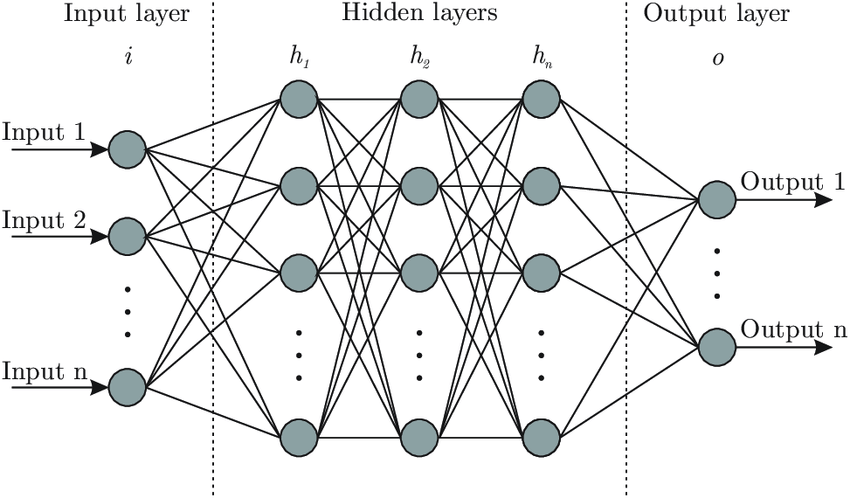
\includegraphics[width=\textwidth]{ANN.png}
    \caption{Architettura di una rete neurale artificiale}
    \label{fig:ANN}
\end{figure}
La rete neurale artificiale (ANN) è un sistema informatico costituito da unità di elaborazione altamente interconnesse tra loro chiamate \textbf{neuroni} (simili ai neuroni biologici nel cervello umano) progettate per replicare le prestazioni di un cervello umano impegnato in un compito particolare. Questi neuroni sono raggruppati in strati o \textbf{livelli}. La struttura ANN più comune (Fig. \ref{fig:ANN}) è costituita da un livello di input, uno o più livelli nascosti e un livello di output. 

Nel cervello umano, i neuroni comunicano inviandosi segnali l'uno all'altro attraverso connessioni complesse. La ANN si basa sullo stesso principio nel tentativo di simulare il processo di apprendimento del cervello umano utilizzando algoritmi complessi. La ANN è ampiamente utilizzata in campo elettrico per la previsione del carico e la previsione del prezzo dell'energia elettrica, questo grazie alla sua capacità di gestire i problemi di relazione non lineare in modo accurato.

\subsection{Modello di un neurone artificiale}
\begin{figure}[h]
    \centering
    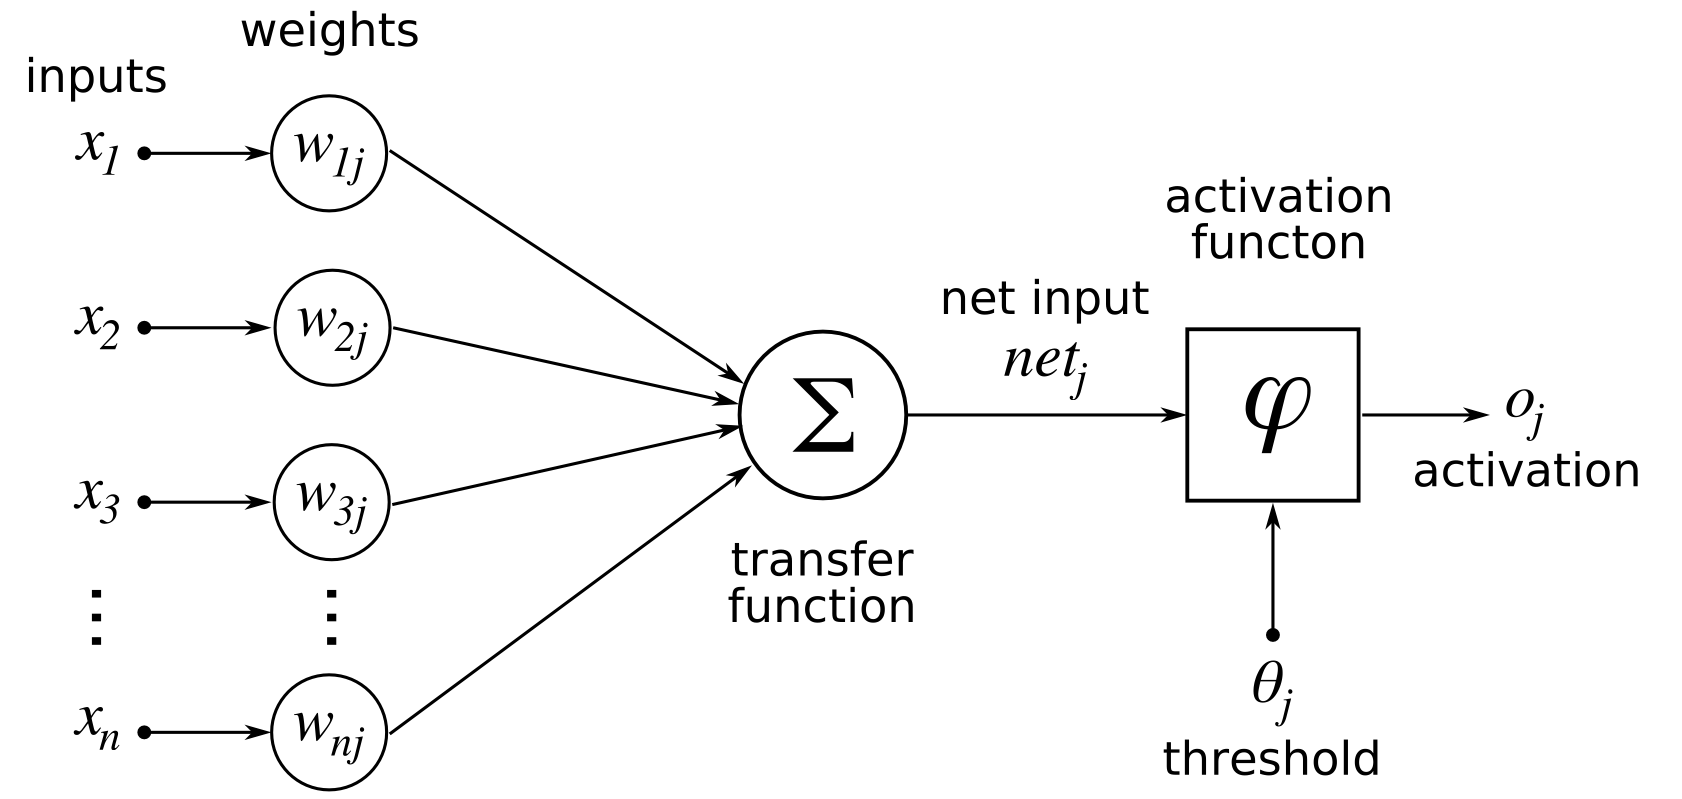
\includegraphics[width=\textwidth]{neurone.png}
    \caption{Modello di un neurone artificiale}
    \label{fig:neurone}
\end{figure}
Un modello semplice di un neurone artificiale è mostrato nella Fig. \ref{fig:neurone}. Viene mostrata una struttura di rete con ingressi ($x_1$, $x_2$, ..., $x_i$) connessi al neurone $j$ con pesi ($w_{1j}$, $w_{2j}$, ..., $w_{ij}$) su ciascuna connessione. Il neurone somma tutti i segnali che riceve, moltiplicando ogni segnale per i pesi associati sulla connessione. Il risultato ($net_j$) viene quindi fatto passare attraverso una funzione di trasferimento (attivazione) che normalmente è non lineare per fornire l'uscita finale $o_j$. La funzione più comunemente usata è la sigmoidea (funzione logistica) per le sue proprietà facilmente differenziabili, che è molto conveniente quando viene applicato l'algoritmo di retropropagazione. 

\subsection{Algoritmo di retropropagazione}
L'algoritmo di retropropagazione funziona riducendo al minimo l'errore tra l'output e il target (reale) propagando l'errore nella rete. I pesi su ciascuna delle connessioni tra i neuroni vengono modificati in base alla dimensione dell'errore iniziale. I dati di input vengono quindi inoltrati nuovamente, producendo un nuovo output ed errore. Il processo viene ripetuto fino a quando non si ottiene un errore minimizzato accettabile. Ciascuno dei neuroni utilizza una funzione di trasferimento ed è completamente connesso ai nodi del livello successivo. Quando l'errore raggiunge un valore accettabile, l'addestramento viene interrotto. Il modello risultante è una funzione che è una rappresentazione interna dell'output in termini di input in quel punto.


\section{Reinforcement Learning}
\label{sec:MARL}
\begin{figure}[h]
    \centering
    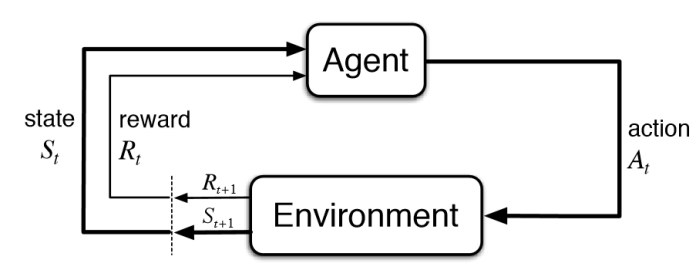
\includegraphics[width=\textwidth]{RL.jpg}
    \caption{Impostazione dell'apprendimento per rinforzo}
    \label{fig:RL}
\end{figure}

L'apprendimento per rinforzo (RL) permette di intraprendere azioni adeguate per massimizzare la ricompensa in una situazione particolare. La Fig. \ref{fig:RL} mostra l'architettura generale di RL. Un \textbf{agente} e il suo \textbf{ambiente} interagiscono tramite una sequenza di fasi temporali discrete e, ad ogni fase, l'agente seleziona \textbf{un'azione} da inviare all'ambiente. Di conseguenza, l'agente ottiene una \textbf{ricompensa} e l'ambiente cambia in un \textbf{nuovo stato}. RL cerca di creare una mappa tra le azioni e gli stati per massimizzare le ricompense totali basandosi sulla conoscenza dell'agente, ottenuta attraverso l'interazione diretta con l'ambiente, in modo incustodito (non supervisionato). 

Grazie all'assenza di modello e nessuna necessità di previa conoscenza del dominio, RL è diventato un potente strumento per ottimizzare il controllo dei sistemi energetici che devono affrontare continui cambiamenti; ad esempio, disponibilità intermittente di risorse rinnovabili, prezzi dinamici dell'elettricità e i cambiamenti negli importi del consumo di energia.


\subsection{Vantaggi dell'apprendimento per rinforzo}
Ci sono molti vantaggi nell'impiego di RL per un processo decisionale ottimale. L'apprendimento per rinforzo gode delle seguenti proprietà:
\begin{description}
\addtolength{\itemindent}{0.5cm}
    \item [Privo di modelli] L'agente non richiede una regola predefinita o una conoscenza preliminare su come selezionare un'azione. Invece, scopre azioni ottimali “imparando” direttamente mentre interagisce con l'ambiente.
    \item [Adattivo] L'agente può acquisire autonomamente le decisioni ottimali, in modo online adattato a diversi apparecchi, tenendo conto dell'incertezza e della flessibilità dell'EMS.
    \item [Conciso] L'intero calcolo si basa su una tabella di consultazione, che è molto più facile da applicare nel mondo reale rispetto ai metodi di ottimizzazione convenzionali.
\end{description}


\subsection{Multi-Agent Reinforcement Learning}
\begin{figure}[h]
    \centering
    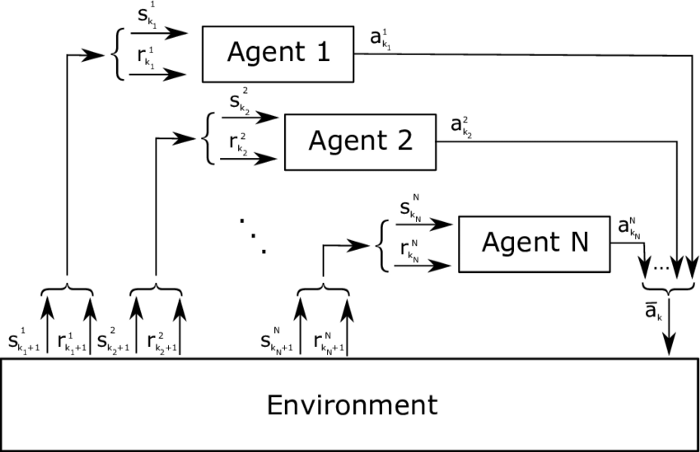
\includegraphics[width=\textwidth]{MARL.png}
    \caption{Impostazione dell’apprendimento per rinforzo multi-agente}
    \label{fig:MARL}
\end{figure}

L'apprendimento per rinforzo multi-agente (MARL) è una complicazione di RL e coinvolge \textbf{numerosi agenti} che operano nello stesso ambiente e spesso collaborando verso un obiettivo finale. Il funzionamento di ogni singolo agente è analogo a quello descritto nell'apprendimento per rinforzo. La caratteristica in questo caso, è che l'ambiente è in grado di fornire ad ogni agente le informazioni richieste; ovvero la ricompenza per l'azione effettuata e il nuovo stato dell'ambiente a seguito di tale azione. 

Quanto detto viene sintetizzato in Fig. \ref{fig:MARL}. MARL trae ispirazione da strutture sociali nel regno animale, si basa anche molto sulla teoria dei giochi. 



\chapter{Background}
\label{cap:3}
L'articolo preso in esame \cite{ref:article} propone un algoritmo di \textbf{Demand Response} (DR) di un'ora in anticipo per più apparecchi in un \textbf{HEMS} che utilizza tecniche di intelligenza artificiale, considerando i costi dell'elettricità e dell'insoddisfazione degli utenti.

In particolare, a causa della natura intrinseca del mercato dei prezzi dell'energia elettrica in anticipo di un'ora, il cliente accede a un solo prezzo per l'ora corrente. Per far fronte all'incertezza dei prezzi futuri, viene presentato un modello di previsione dei prezzi stabile, che viene implementato da una \textbf{rete neurale artificiale} (ANN). La previsione dei prezzi è diventato un argomento importante nell'ingegneria elettrica degli ultimi anni e sono stati tentati diversi metodi di implementazione. L'approccio ANN è relativamente facile da implementare e mostra buone prestazioni, essendo meno dispendioso in termini di tempo rispetto ad altre tecniche. Ogni volta che si ottiene il nuovo prezzo dell'elettricità, il modello ANN prevede i prezzi futuri e questo processo si ripete ogni ora fino alla fine della giornata. 

Inoltre, in collaborazione con i prezzi futuri previsti, viene adottato un algoritmo di \textbf{apprendimento per rinforzo multi-agente} (MARL) per prendere decisioni ottimali per diversi apparecchi in modo decentralizzato, per ridurre al minimo la bolletta energetica dell'utente e il grado di disservizio. Qui, ogni apparecchio ha un agente e RL viene utilizzato per il processo decisionale nel contesto dell'incertezza relativa alle informazioni sui prezzi e alla domanda di carico degli apparecchi. In tal modo, il carico computazionale viene spostato da un ottimizzatore centrale a un insieme di agenti intelligenti che arrivano collettivamente a una soluzione ottimale. 

\section{Previsione dei prezzi con ANN}
Nel modello di previsione dei prezzi di questo problema, gli \textbf{input dettagliati} sono elencati nella Tab. \ref{tab:ANN} e l'output è rappresentato dai prezzi previsti. In generale, i parametri di prezzo possono dipendere da diversi fattori. In particolare, dipendono sia dai prezzi storici dell'elettricità a breve che a lungo termine e dalla domanda di energia. Inoltre, i primi tre input sono utili, in quanto i prezzi possono variare se un giorno è festivo o meno, a seconda dell'ora del giorno e a seconda che si tratti di una giornata lavorativa o del fine settimana.

Viene adottata la \textbf{funzione Sigmoidea} come funzione di trasferimento di ogni livello e \textbf{l'algoritmo Levenberg-Marquardt} viene utilizzato come algoritmo di training per il modello. Le prestazioni di questo modello sono valutate \textbf{mediante errore assoluto medio} (MAE) e \textbf{errore percentuale assoluto medio} (MAPE) tra i valori previsti e effettivi. Questi sono mostrati nelle Eq. \ref{eq:MAE} e \ref{eq:MAPE}:
\begin{equation}
\label{eq:MAE}
    MAE = \frac{1}{T} \sum^{T}_{t=1} \left| RTP_t - RTP^{f}_{t} \right|
\end{equation}
\begin{equation}
\label{eq:MAPE}
    MAPE = \frac{100}{T} \sum^{T}_{t=1} \frac{\left| RTP_t - RTP^{f}_{t} \right|}{RTP_t}
\end{equation}
dove $RTP_t$ rappresenta il prezzo effettivo e $RTP^{f}_{t}$ indica il prezzo previsto.

\begin{table}[h]
    \center
    \caption{Inputs della rete neurale artificiale}
    \label{tab:ANN}
    \begin{tabular}{c|l}
        \hline
        \hline
        Input index & Description \\
        \hline
        1 & Day of week (1-7) \\
        \hline
        2 & Hour stage of day (1-24) \\
        \hline
        3 & Is holiday (0 or 1) \\
        \hline
        4 & Electricity demand of hour $h-1$ \\
        \hline
        5 & Electricity demand of hour $h-2$ \\
        \hline
        6 & Electricity demand of hour $h-3$ \\
        \hline
        7 & Electricity demand of hour $h-24$ \\
        \hline
        8 & Electricity demand of hour $h-25$ \\
        \hline
        9 & Electricity demand of hour $h-26$ \\
        \hline
        10 & Hour-ahead price of hour $h-1$ \\
        \hline
        11 & Hour-ahead price of hour $h-2$ \\
        \hline
        12 & Hour-ahead price of hour $h-3$ \\
        \hline
        13 & Hour-ahead price of hour $h-24$ \\
        \hline
        14 & Hour-ahead price of hour $h-25$ \\
        \hline
        15 & Hour-ahead price of hour $h-26$ \\
        \hline
        16 & Hour-ahead price of hour $h-48$ \\
        \hline
        17 & Hour-ahead price of hour $h-49$ \\
        \hline
        18 & Hour-ahead price of hour $h-50$ \\
        \hline
        \hline
    \end{tabular}
\end{table}


\section{Processo decisionale con MARL}
Per eseguire un'azione ottimale, il problema è modellato come un orizzonte temporale discreto tramite \textbf{processi decisionali di Markov} (MDP), e gode quindi della proprietà di Markov secondo la quale le transizioni di stato dipendono solo dallo stato corrente e dall'azione corrente intrapresa e, quindi, sono indipendenti da tutti i precedenti stati ambientali e azioni degli agenti. 

Gli \textbf{elementi chiave} di questo modello sono i seguenti:
\begin{itemize}
    \item un'ora discreta $h$;
    \item un'azione $a_h$;
    \item uno stato $s_h$;
    \item una ricompensa $r(s_h, a_h)$.
\end{itemize}
Viene usato $\upsilon$ per indicare la politica di mappatura degli stati sulle azioni, ad es. $\upsilon:a_h=\upsilon(s_h)$. L'obiettivo di questo problema RL è scoprire una \textbf{politica ottimale} per ogni stato $s_h$ in modo che l'azione $a_h$ selezionata massimizzi la ricompensa $r(s_h, a_h)$.

Per ottenere la politica ottimale viene usato il \textbf{Q-learning}, una tecnica di RL. Il meccanismo alla base del Q-learning è l'assegnazione di un Q-value $Q(s_h, a_h)$ a ciascuna coppia stato-azione all'ora $h$ e l'aggiornamento di questo valore ad ogni iterazione, in modo da ottimizzare la ricompensa. Il Q-value ottimale $Q^{\ast}_\upsilon(sh, ah)$, indica la ricompensa futura massima $r(s_h, a_h)$ quando si intraprende un'azione $a_h$ allo stato $s_h$ mentre si continua a seguire la politica ottimale $\upsilon$, che soddisfa \textbf{l'equazione di Bellman} di seguito:
\begin{equation}
\label{eq:bellman}
Q^{\ast}_\upsilon(s_h, a_h)=r(s_h,a_h)+\gamma \cdot \max Q(s_{h+1}, a_{h+1})
\end{equation}
dove $\gamma \in [0,1]$  è un fattore di attualizzazione che indica l'importanza relativa dei premi futuri rispetto a quelli attuali. 

Ogni ora, un agente esegue un'azione e il Q-value della cella corrispondente viene aggiornato in base all'equazione di Bellman, Eq. \ref{eq:bellman}, come segue:
\begin{equation}
    Q(s_h, a_h) \leftarrow Q(s_h, a_h)+\theta[r(s_h, a_h)+\gamma \cdot \max Q(s_{h+1}, a_{h+1})-Q(s_h, a_h)]
\end{equation}
dove $\theta \in [0,1]$ è il tasso di apprendimento che rappresenta in che misura il nuovo Q-value prevale sui vecchi.

In un \textbf{contesto multi-agente}, ciascun agente agisce in modo indipendente per identificare la sua politica ottimale. Durante il processo di apprendimento, ciascun agente mantiene i propri Q-value e raggiunge una politica basata esclusivamente sugli effetti che si verificano nell'ambiente causati dalle proprie azioni. Ogni politica è implementata come un processo di Q-learning separato. Quando ogni agente raggiunge il Q-value ottimale, tutti gli agenti hanno ottenuto la massima ricompensa, il che significa che anche la somma dei premi è al massimo e il sistema ha raggiunto il \textbf{Q-value globale ottimale}.

Nel problema descritto ogni elettrodomestico rappresenta un ambiente e ognuno ha il proprio agente. I singoli agenti del sistema possono essere modellati nelle tre tipologie descritte in seguito.

\subsection{Carico non spostabile}
I carichi non spostabili hanno \textbf{richieste di consumo di energia che devono essere assolutamente soddisfatte}, ad esempio i \textbf{frigoriferi} (REFG) o alcuni sistemi di sicurezza. Una volta che un carico non spostabile inizia a funzionare, deve \textbf{funzionare continuativamente} e non può essere arrestato. Il consumo di energia di tali carichi è sempre uguale alle loro richieste di consumo di energia:
\begin{equation}
    E^{non}_{n,h} = e^{non}_{n,h}
\end{equation}
Il costo di questo tipo di apparecchio è solo la bolletta dell’elettricità per il consumo di energia. Pertanto, la funzione di utilità dei carichi non spostabili è:
\begin{equation}
    U^{non}_{n,h} = P_h \cdot E^{non}_{n,h}
\end{equation}
dove $P_h$ indica il prezzo dell'elettricità all'ora $h$.

\subsection{Carico spostabile}
I carichi spostabili possono \textbf{programmare la loro richiesta di consumo di energia} per beneficiare delle ore in cui i prezzi sono bassi, in modo da evitare i picchi di consumo di energia e ridurre la bolletta energetica. Ad esempio, le \textbf{lavatrici} (WM) solitamente funzionano durante un periodo di lavoro $[T_{n,ini}, T_{n,end}]$ e richiedono di \textbf{funzionare continuativamente per una durata $T_{n,ne}$} per completare le loro operazioni. Tipicamente il carico spostabile ha due azioni disponibili: “on” e “off”. Il consumo di energia di tali carichi è il seguente:
\begin{equation}
    E^{shift}_{n,h} = I_{n,h} \cdot e^{shift}_{n,h}
\end{equation}
dove $I_{n,h}$ è una variabile binaria: $I_{n,h} = 1$ se l'apparecchio $n$ lavora all'ora $h$; $I_{n,h} = 0$ altrimenti. Per questo tipo di apparecchio esistono due tipi di costi: la bolletta dell'elettricità per il consumo di energia e l'insoddisfazione dei tempi di attesa prima che un dispositivo inizi e poi completi il suo funzionamento. Pertanto, la funzione di utilità di un carico spostabile è:
\begin{equation}
\label{eq:shift U}
    U^{shift}_{n,h} = P_h \cdot E^{shift}_{n,h}+k_n \cdot (T_{n,w}-T_{n,ini})
\end{equation}
\begin{equation}
    T_{n,ini} \leq T_{n,w} \leq [T_{n,end}-T_{n,ne}]
\end{equation}
\begin{equation}
    T_{n,ne} \leq T_{n,end}-T_{n,ini}
\end{equation}
dove $T_{n,w}$ è l'ora in cui il carico inizia a lavorare, quindi il tempo di attesa sarebbe $T_{n,w} - T_{n,ini}$, e $k_n$ è un coefficiente che dipende dal dispositivo. Il primo termine dell'Eq. \ref{eq:shift U} rappresenta il costo dell'elettricità e il secondo termine indica il costo del tempo di attesa.

\subsection{Carico controllabile}
I carichi controllabili possono essere gestiti con un \textbf{consumo di energia flessibile} tra la richiesta minima di consumo di energia e la richiesta massima, indicate rispettivamente da $e_{n,min}$ e $e_{n,max}$. Ad esempio, i \textbf{condizionatori d'aria} (AC) possono \textbf{regolare il loro consumo di energia} da $e_{n,min}$ a $e_{n,max}$ in risposta alle variazioni di prezzo. Il consumo di energia dei carichi controllabili è:
\begin{equation}
    E^{con}_{n,h} = e^{con}_{n,h}
\end{equation}
\begin{equation}
    e_{n,min} \leq e^{con}_{n,h} \leq e_{n,max}
\end{equation}
L'obiettivo di questo tipo di apparecchio è ridurre al minimo la bolletta dell'elettricità per il consumo di energia, diminuendo la richiesta di energia durante le ore critiche, tuttavia, la potenza ridotta può causare insoddisfazione per l'utente. Pertanto, la funzione di utilità di un dispositivo controllabile $n$ è:
\begin{equation}
    U^{con}_{n,h} = P_h \cdot E^{con}_{n,h} + \beta_n \cdot (E^{con}_{n,h} - e_{n,max})^2
\end{equation}
dove $\beta_n$ è un parametro di costo di insoddisfazione dipendente dal dispositivo. Il primo termine indica il costo dell'elettricità e il secondo termine indica il costo dell'insoddisfazione dell'utente, definito da una funzione quadratica.

\subsection{Funzione obiettivo}
La funzione obiettivo ha il compito di minimizzare il costo dell'elettricità, ma anche di minimizzare il costo dell'insoddisfazione dell'utente. Può quindi essere espressa come segue:
\begin{equation}
    \begin{split}
    \min \sum^{N}_{n=1} \sum^{H}_{h=1} \Bigg\{ \Big(1-\rho\Big) \cdot P_h \cdot \Big( E^{non}_{n,h} + E^{shift}_{n,h} + E^{con}_{n,h} \Big) + \\ \rho \cdot \bigg[ k_n \cdot \Big(T_{n,w} - T_{n,ini}\Big) + \beta_n \cdot \Big(E^{con}_{n,h} - e_{n,max}\Big)^2\bigg] \Bigg\}
    \end{split}
\end{equation}
Il primo termine indica il costo dell'elettricità e il secondo termine indica il costo dell'insoddisfazione. $\rho$ è un parametro di equilibrio.

\section{Combinazione di ANN e MARL}
La Fig. \ref{fig:architettura} mostra nel dettaglio l'algoritmo DR che combina ANN e MARL: ogni ora l'HEMS riceve il prezzo dell'elettricità di un'ora in anticipo e utilizza la rete neurale artificiale per prevedere i prezzi futuri. Quindi, viene adottato l'apprendimento per rinforzo multi-agente per ottenere le decisioni ottimali per i diversi tipi di elettrodomestici.

\begin{figure}[h]
    \centering
    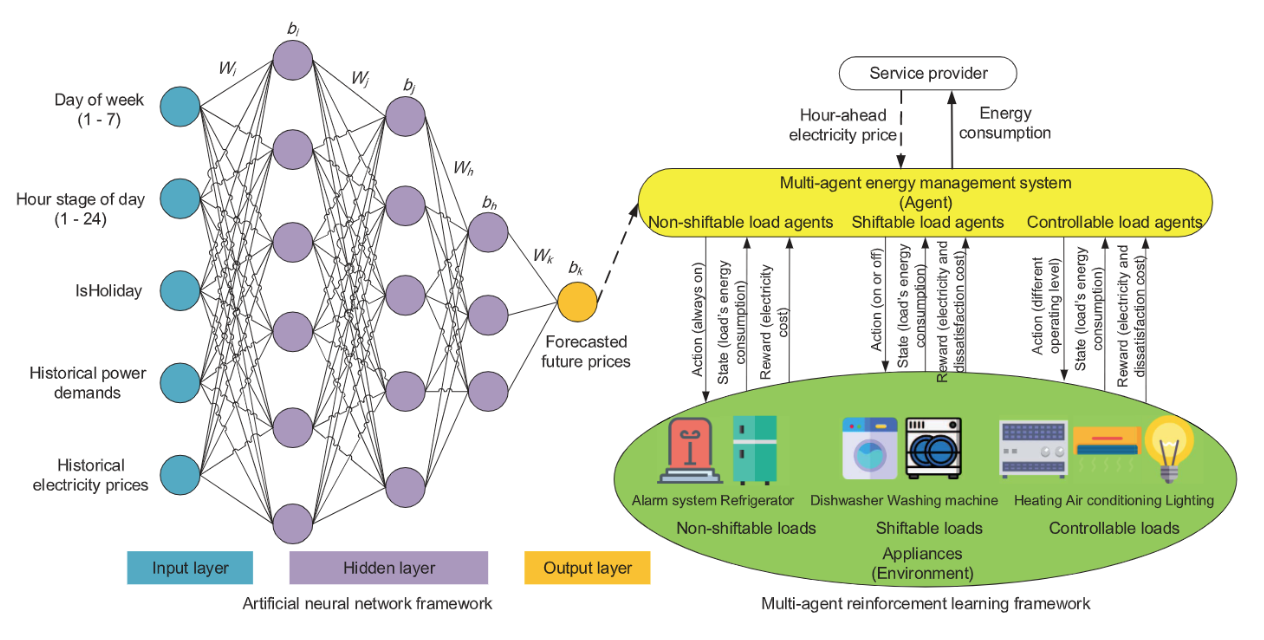
\includegraphics[width=\textwidth]{Architettura ANN MARL.png}
    \caption{Combinazione di ANN e MARL}
    \label{fig:architettura}
\end{figure}


\chapter{Miglioramenti dell'approccio}
\label{cap:4}
\section{Integrazione di un veicolo elettrico plug-in}
Un veicolo elettrico plug-in (PEV) dispone di una batteria interna capace di essere caricata esternamente, cioè in una stazione di ricarica o grazie a una normale presa di corrente. Negli anni la capacità delle batterie è aumentata in modo esponenziale, al punto da dare ai guidatori di PEV sempre più autonomia. 

Di seguito viene descritta una strategia di gestione della carica di un PEV con alimentazione modulabile, al fine di \textbf{integrare la carica del PEV nell'HEMS descritto precedentemente}. Occorre quindi capire come modellare il PEV partendo delle tre tipologie di elettrodomestico prima descritte (carico non spostabile, carico spostabile, carico controllabile).


\subsection{Tipologie di modellazione del PEV}
\label{subsec:tipmod}
È possibile modellare il PEV come se fosse una batteria da caricare connessa all'impianto elettrico dell'abitazione. Questo comporta che l'agente associato al PEV prenda in considerazione alcuni aspetti che non sono ancora stati definiti, ovvero lo \textbf{stato di carica} della batteria, e la \textbf{capacità massima} di quest'ultima. Quindi l'agente preposto a prendere decisioni circa la carica della batteria del PEV, deve rispettare i seguenti vincoli:
\begin{equation}
\label{eq:vincolo1}
0 \leq SOC_{b,h} \leq C_b
\end{equation}
\begin{equation}
\label{eq:vincolo2}
0 \leq E_{b,h} \leq C_b - SOC_{b,h-1}
\end{equation}
\begin{equation}
\label{eq:vincolo3}
SOC_{b,h} = SOC_{b,h-1} + E_{b,h-1}
\end{equation}
dove $b$ è la batteria del PEV, $SOC_{b,h}$ e $C_b$ sono rispettivamente lo stato di carica della batteria del PEV alla fine dell'ora $h$, e la capacità massima della batteria del PEV. $E_{b,h}$ è la richiesta di consumo di energia di $b$ all'ora $h$.

Di seguito vengono descritte tutte le modellazioni della batteria del PEV prese in esame.

\subsubsection{Carico non spostabile}
La batteria del PEV può essere modellata come un carico non spostabile siccome è possibile caricarla appena viene attaccata all'abitazione, e smettere di caricarla quando il suo stato di carica ha raggiunto la capacità massima, oppure quando il PEV viene staccato dall'abitazione.
Il consumo di energia della batteria come carico non spostabile, prendendo atto dei vincoli della batteria, è il seguente:
\begin{equation}
E^{non}_{b,h} = \min(e^{non}_{b,h}, C_b - SOC_{b,h-1})
\end{equation}
La funzione di utilità della batteria come carico non spostabile è quindi la seguente:
\begin{equation}
U^{non}_{b,h} = P_h \cdot E^{non}_{b,h}
\end{equation}

Questa tipologia di modellazione garantisce priorità assoluta alla carica della batteria, ma non permette di prendere decisioni al fine di contribuire a ridurre i picchi di domanda dell'abitazione. Considerato il peso che ha la carica del PEV su di un'abitazione, è consigliabile provare a modellare la sua batteria in altro modo. 

\subsubsection{Carico spostabile}
La batteria del PEV può completare la sua carica pianificandola nell'intervallo di tempo $[T_{n,ini}, T_{n,end}]$. Il consumo di energia della batteria come carico spostabile, prendendo atto dei vincoli della batteria, è il seguente:
\begin{equation}
E^{shift}_{b,h} = I_{b,h} \cdot \min(e^{shift}_{b,h}, C_b - SOC_{b,h-1})
\end{equation}
La funzione di utilità della batteria come carico spostabile è quindi la seguente:
\begin{equation}
    U^{shift}_{b,h} = P_h \cdot E^{shift}_{b,h}+k_b \cdot (T_{b,w}-T_{b,ini})
\end{equation}
\begin{equation}
    T_{b,ini} \leq T_{b,w} \leq [T_{b,end}-T_{b,ne}]
\end{equation}
\begin{equation}
    T_{b,ne} = \min \Bigg( \Bigg \lceil \frac{C_b - SOC_{b,h-1}}{e^{shift}_{b,h}} \Bigg \rceil, T_{b,end}-T_{b,ini} \Bigg)
\end{equation}
Da notare che conoscendo lo stato di carica e la capacità massima della batteria, $T_{b,ne}$ è ben definito. 

La modellazione tramite carico spostabile garantisce che la batteria venga caricata al pari di una modellazione tramite carico non spostabile. La differenza è che la carica non ha però la priorità assoluta, perchè il carico spostabile programma l'intervallo di ore in cui lavorare, al fine di caricare la batteria in quello ottimale secondo l'algoritmo MARL.

Questa modellazione assume che venga definita $T_{b,end}$ all'ora $T_{b,ini}$ e quindi per il corretto funzionamento del processo decisionale del carico spostabile, la batteria deve essere collegata all'abitazione, nel caso peggiore, per tutto l'intervallo $[T_{b,ini}, T_{b,end}]$. Significa quindi che il PEV non è disponibile per un periodo di tempo anche maggiore di $T_{b,ne}$. Aumentando il valore $k_b$ questa criticità si riduce, ma viene meno il risparmio sul costo dell'energia.

Se comunque si è disposti a tollerare questa inefficienza a fronte di un risparmio sulla bolletta dell'elettricità, è possibile modellare la batteria del PEV in un modo alternativo (carico spostabile e divisibile), prendendo spunto dal carico spostabile e facendo uso di una proprietà di cui la batteria può godere a differenza di carichi spostabili come la lavatrice.

\subsubsection{Carico spostabile e divisibile}
La seguente tipologia di modellazione della batteria del PEV ha senso di esistere grazie alla possibilità, da parte della batteria, di programmare e quindi posticipare la sua carica, ma anche e soprattutto grazie alla possibilità di \textbf{suddividere la carica in più intervalli distinti}. Quest'ultima proprietà non appartiene ai carichi spostabili che, per definizione, una volta avviati devono funzionare continuativamente per la durata $T_{b,ne}$. Questa osservazione permette quindi di modellare la batteria del PEV come carico spostabile e divisibile.

Il processo decisionale di questa tipologia non fa uso dell'apprendimento per rinforzo multi-agente, ma bensì di un algoritmo “naïf” che fa unicamente affidamento ai prezzi futuri previsti da ANN. L'idea alla base dell'algoritmo è quella di caricare la batteria nelle ore dell'intervallo $[T_{b,ini}, T_{b,end}]$ dove il prezzo dell'elettricità è minore secondo i prezzi futuri previsti. Di questa tipologia è di interesse sapere il consumo di energia, $T_{ne}$ e l'intervallo $[T_{b,ini}, T_{b,end}]$.
\begin{equation}
E^{naïf}_{b,h} = I_{b,h} \cdot \min(e^{naïf}_{b,h}, C_b - SOC_{b,h-1})
\end{equation}
\begin{equation}
    T_{b,ne} = \min \Bigg( \Bigg \lceil \frac{C_b - SOC_{b,h-1}}{e^{naïf}_{b,h}} \Bigg \rceil, T_{b,end}-T_{b,ini} \Bigg)
\end{equation}
Modellare la batteria del PEV come carico spostabile e divisibile è un'ottima scelta quando si vuole puntare a ridurre il costo della bolletta e si è tollera l'indisponibilità del PEV durante $[T_{b,ini}, T_{b,end}]$.

\subsubsection{Carico controllabile}
L'ultima tipologia presa in esame è quella che permette di modellare la batteria del PEV come un carico controllabile. Questa tipologia ha una maggiore flessibilità rispetto ai carichi spostabili per quanto riguarda la modulazione della richiesta di consumo di energia, ma meno flessibilità rispetto ai carichi spostabili e divisibili. Rispetto a questi ultimi però, questa modellazione ha una maggiore flessibilità riguardo alla disponibilità del PEV. Infatti, modellando la batteria del PEV come un carico controllabile, il PEV non è soggetto ad alcuna indisponibilità. Resta ragionevolmente il disservizio dell'utente, presente nella funzione di unità.

Il consumo di energia della batteria come carico controlabile, prendendo atto dei vincoli della batteria, è il seguente:
\begin{equation}
E^{con}_{b,h} = e^{con}_{b,h}
\end{equation}
\begin{equation}
0 \leq e^{con}_{b,h} \leq \min(e_{b,max}, C_b - SOC_{b,h-1})
\end{equation}
La funzione di utilità della batteria come carico controllabile è quindi la seguente:
\begin{equation}
    U^{con}_{b,h} = P_h \cdot E^{con}_{b,h} + \beta_b \cdot (E^{con}_{b,h} - \min(e_{b,max}, C_b - SOC_{b,h-1}))^2
\end{equation}
\section{Modifiche apportate all'algoritmo MARL}
Nella seguente sezione si discutono le modifiche apportate all'algoritmo MARL dell'HEMS, effettuate per quanto riguarda l'integrazione della carica del PEV nell'algoritmo stesso. Tali modifiche sono argomentate e giustificate in seguito, e sono state apportate per motivi di semplificazione e necessità, o talvolta a causa di poca chiarezza da parte dell'articolo preso in esame. Così, a fronte di valutazioni e considerazioni, si è preferito apportare alcune modifiche a favore di soluzioni più chiare, versatili, esplicative e semplici.




\subsection{Stati delle Q-table}
\label{sec:stati}
Nell'articolo preso in esame, gli stati delle Q-table sono indicati dalle informazioni sul consumo di energia degli apparecchi. Nell'articolo però è evidente come le ore giochino un ruolo fondamentale nella divisione discreta del modello decisionale. Infatti si ricorda che il problema stesso è modellato come un orizzonte temporale discreto tramite processi decisionali di Markov. Si noti che le ore stesse possono essere considerate come stati delle Q-table, anche perchè la definizione di stati data dall'articolo è poco chiara e sbrigativa. Tutt'al più il problema viene modellato discretamente tramite intervalli orari, quindi comunque le ore sono una dimensione delle Q-table. Là dove non è chiaro chi svolga il ruolo degli stati, è possibile farlo svolgere alle ore, anche perchè, indentificare gli stati in un modo diverso dalle ore, significherebbe generare Q-table di tre dimensioni (ore, stati, azioni) rendendo più difficile il processo di apprendimento per rinforzo.

Seguendo questi ragionamenti, nella Q-table della batteria del PEV, modellata come carico spostabile, gli stati sono identificati dalle ore, generando così una Q-table di due dimensioni e rendendo quindi l'apprendimento più efficace. Questa scelta è supportata dal fatto che, modellando la Q-table come descritto, i valori in quest'ultima vengono memorizzati in celle che dipendono dalle ore e dalle azioni, che sono proprio le dipendenze sulle quali si basa la funzione di unità dei carichi spostabili. Quindi ci si può convincere che i valori inseriti nella Q-table sono suddivisi e totalizzati tra loro nel modo corretto, per un chiaro apprendimento.

Per la Q-table della batteria del PEV, modellata come carico controllabile, è possibile applicare un ragionamento analogo a quello appena formulato. Si noti che la funzione di unità di questa modellazione è dipendente dalle ore, dalle azioni, ma anche dallo stato di carica della batteria. Per questo motivo si è scelto di generare, per la batteria del PEV, modellata come carico controllabile, una Q-table di tre dimensioni (ore, stati, azioni), dove gli stati sono definiti in base allo stato di carica della batteria.

Per verificare la correttezza di queste formulazioni, sono state messe a confronto le prestazioni di due batterie modellate come carico spostabile aventi: la prima, una Q-table a tre dimensioni (ore, stati di carica, azioni); la seconda, una Q-table a due dimensioni (ore, azioni). L'esito del confronto ha visto la Q-table bidimensionale performare meglio, confermando la tesi.

Infine sono state messe a confronto le prestazioni di due batterie modellate come carico controllabile aventi: la prima, una Q-table a tre dimensioni (ore, stati di carica, azioni); la seconda, una Q-table a due dimensioni (ore, azioni). L'esito del confronto ha visto la Q-table tridimensionale performare meglio, confermando la tesi.

\subsubsection{Stati iniziali}
Definiamo quali sono gli stati iniziali per le Q-table delle batterie implementate come carico spostabile e per quelle implementate come carico controllabile. La definizione data è analoga per entrambe le tipologie di modellazione ed è la seguente: gli stati iniziali sono quelli in cui la batteria si trova all'inizio dell'ora nella quale si deve effettuare un processo decisionale. 

\subsubsection{Stati finali}
Per quanto riguarda gli stati finali, questi sono definibili genericamente come segue: gli stati finali sono quelli i cui la batteria ha completato la carica, ovvero quando lo stato di carica della batteria è equivalente alla sua capacità massima.




\subsection{Convergenza delle Q-table}
Nell'articolo preso in esame il criterio di terminazione dell'apprendimento orario è calcolato come $\left|Q^i-Q^{i-1}\right|\leq \phi$. Se la differenza tra $Q^i$ e $Q^{i-1}$ non è maggiore di $\phi$, la $Q^i$ converge al valore massimo; il che vuol dire che si è raggiunta una politica ottimale. $\phi$ è un parametro di piccola dimensione che dipendente dal sistema. L'algoritmo RL dell'articolo è quindi il seguente (Alg. \ref{alg:1}):

\begin{figure}[ht]
    \centering
    \begin{minipage}{\linewidth}
        \begin{algorithm}[H]
        \label{alg:1}
            \SetAlgoLined
            Initialize $Q(s,a)$\;
            \While{Q-value is converged, such that $\left|Q^i-Q^{i-1}\right|\leq \phi$}{
                Initialize $s$ to initial state\;
                \While{$s$ != final state}{
                Choose a from s using $\varepsilon$-greedy policy\;
                Take action $a$, observe reward $r(s, a)$ and next state $s'$\;
                $Q(s, a) \leftarrow Q(s, a)+\theta[r(s, a)+\gamma \cdot \max Q(s', a')-Q(s, a)]$\;
                }
            }
            \caption{Algoritmo di Q-learning con convergenza di Q-table}
        \end{algorithm}
    \end{minipage}
\end{figure}

La  convergenza  degli  algoritimi di apprendimento per rinforzo può essere però molto lenta, soprattutto in ambienti dinamici. Un ambiente reale risulta nella maggior parte dei casi molto  dinamico. L’apprendimento  per rinforzo non riuscirebbe, perciò, a convergere verso una politica ottimale a causa dei continui cambiamenti dell’ambiente. È proprio questo il caso della batteria del PEV. Quest'ultima, a causa della sua consistente richiesta di consumo di energia, rende l'ambiente molto dinamico e quindi rende difficile la convergenza delle Q-table; e lungo il processo di apprendimento.

Per questo motivo, si è scelto di adottare una differente tipologia di convergenza per decretare termitato il processo di apprendimento dell'agente. Nell'implementazione della batteria del PEV viene adottata la convergenza lieare. Questa consiste nell'iterare l'apprendimento per un determinato numero di volte (episode). L'algoritmo che fa uso di tale convergenza, e anche quello utilizzato per l'implementazione della batteria, è il seguente (Alg. \ref{alg:2}):

\begin{figure}[ht]
    \centering
    \begin{minipage}{\linewidth}
        \begin{algorithm}[H]
        \label{alg:2}
            \SetAlgoLined
            Initialize $Q(s,a)$\;
            \For{each episode}{
                Initialize $s$ to initial state\;
                \While{$s$ != final state}{
                Choose a from s using $\varepsilon$-greedy policy\;
                Take action $a$, observe reward $r(s, a)$ and next state $s'$\;
                $Q(s, a) \leftarrow Q(s, a)+\theta[r(s, a)+\gamma \cdot \max Q(s', a')-Q(s, a)]$\;
                }
            }
            \caption{Algoritmo di Q-learning con convergenza lineare}
        \end{algorithm}
    \end{minipage}
\end{figure}

Per verificare la correttezza di questa decisione presa, è stata comunque implementata la batteria mediante Alg. \ref{alg:1}, ma l'elevata dinamicità dell'ambiente non ha reso possibile ottenere la convergenza tra $Q^i$ e $Q^{i-1}$. Si conferma, quindi, un'ottima sostituta la convergenza lieare, utile alla nostra implementazione. 




\subsection{Quando inizializzare le Q-table?}
Nell'HEMS che fa uso di MARL, gli agenti devono svolgere ogni ora l'azione ottimale secondo la politica che hanno formulato all'inizio di quell'ora stessa. Gli agenti quindi, iniziano il loro processo di apprendimento all'inizio dell'ora di interesse, per poter poi eseguire l'azione ottimale. Questo processo inizia da una Q-table con tutti valori inizializzati a zero, per poi riempire i valori di questa Q-table, in modo che, terminati gli episode di apprendimento, l'agente sia in grado di effettuare l'azione ottimale, indicata dalla politica generata dalla Q-table. Questo processo descritto ha inizio e fine nella stessa ora, e quindi, i valori acquisiti nella Q-table vengono cancellati una volta terminati gli episode e scelta l'azione ottimale per quell'ora. L'ora successiva il tutto si ripete.

Abbiamo prima verificato che, a causa dell'elevata dinamicità dell'ambiente, a volte è impossibile raggiungere la convergenza per ottenere una politica realmente ottimale. Ed ora abbiamo appena descritto che ogni tabella è fine all'ora di sua competenza. Potremmo quindi ben pensare di mantenere i valori acquisiti nella Q-table in un'ora, e proseguire l'apprendimento dell'ora successiva sulla tabella dell'ora precedente.

Questa idea è stata contemplata nell'implementazione effettuata al capitolo successivo. È quindi possibile, se si vuole, decidere per quante ore mantenere la stessa Q-table prima di azzerarne i valori; a fronte di un nuovo apprentimento da una Q-table completamente azzerata nei valori. 

Sono state fatte delle valutazioni mantenendo, per tutto il corso di apprendimento di un anno, la stessa Q-table. L'esito va a degenerare nelle prestazioni a causa di alcune tendenze errate che la Q-table può intarprendere dopo parecchie iterazioni di apprendimento. È consigliabile quindi non mantenere la stessa Q-table a lungo termine. 

Nell'implementazione sviluppata, così come nell'articolo preso in esame, le Q-table hanno la durata di un'ora, il che vuol dire che sviluppano un processo di apprendimento al fine unico di scegliere l'azione ottimale per la singola ora di loro competenza.





\chapter{Implementazione}
\label{cap:5}
In questo capitolo verranno illustrate le implementazioni delle tipologie di modellazione per la batteria di un PEV, discusse nella Sec. \ref{subsec:tipmod}. Verranno descritte le variabili e le funzioni di maggior rilievo. Per visionare il codice sorgente completo si faccia riferimento alla repository GitHub \cite{ref:github}.


\section{Non-Shiftable Battery}

\begin{minted}[fontsize=\footnotesize,frame=single,linenos,numbersep=-14pt,breaklines]{python}
    class Non_Shiftable_load(object):
    
        def __init__(self, name, energy_demand):
            self.name = name
            self.is_on = False
            self.energy_demand = energy_demand
            self.filename = os.path.join(directory, str(self.name) + ".csv")
            self.initialize_file()
            return
\end{minted}
\begin{minted}[fontsize=\footnotesize,frame=single,linenos,numbersep=-14pt,breaklines]{python}
    class NSL_Battery(Non_Shiftable_load):
    
        def __init__(self, name, energy_demand, state_of_charge, max_capacity):
            Non_Shiftable_load.__init__(self, name, energy_demand)
            self.state_of_charge = state_of_charge
            self.max_capacity = max_capacity
            return
\end{minted}
\begin{minted}[fontsize=\footnotesize,frame=single,linenos,numbersep=-14pt,breaklines]{python}
    def function(self):
        time = datetime.datetime.now()
        E = 0.0
        U = 0.0
        if self.is_on:
            E = min(self.energy_demand, self.max_capacity - self.state_of_charge)
            U = (1 - rho) * array_price[0] * E
            self.state_of_charge += E
        time = datetime.datetime.now() - time
        self.update_history(E, U, time)
        return E, U
\end{minted}
Questa implementazione non gode dei vantaggi decisionali ottenuti tramite apprendimento per rinforzo, infatti si limita a caricare la batteria ogni qualvolta questa sia collegata alla rete elettrica dell'abitazione (ovvero quando \texttt{self.is\_on == True}).
\section{Shiftable Battery}
\begin{minted}[fontsize=\footnotesize,frame=single,linenos,numbersep=-14pt,breaklines]{python}
    class Shiftable_load(object):
    
        def __init__(self, name, k, Tini, Tend, Tne, energy_demand, state_number):
            self.name = name
            self.is_on = False
            self.k = k
            self.Tini = Tini
            self.Tend = Tend 
            self.Tne = Tne 
            self.energy_demand = energy_demand
            self.state_number = state_number
            self.Tw = -1 
            self.hours_available = -1 
            self.hours_worked = -1 
            self.Q = np.zeros((24, self.state_number, 2), dtype=float)
            self.filename = os.path.join(directory, str(self.name) + ".csv")
            self.initialize_file()
            return
\end{minted}



\begin{minted}[fontsize=\footnotesize,frame=single,linenos,numbersep=-14pt,breaklines]{python}
    class SL_Battery(Shiftable_load):
    
        def __init__(self, name, k, Tini, Tend, Tne, energy_demand, state_number, state_of_charge, max_capacity): 
            Shiftable_load.__init__(self, name, k, Tini, Tend, Tne, energy_demand, state_number)
            self.state_of_charge = state_of_charge
            self.max_capacity = max_capacity
            return
\end{minted}

Di seguito alcuni chiarimenti: 
\begin{itemize}

    \item \textbf{\texttt{self.hours\_available}} indica il totale delle ore disponibili per effettuare la carica (per costruzione \texttt{self.hours\_available = min(self.Tend - self.Tini, self.Tend - current\_hour)});
    \item \textbf{\texttt{self.hours\_worked}} è il contatore delle ore che la batteria ha svolto (obiettivo: raggiungere le \texttt{Tne} ore di lavoro);
    \begin{itemize}
        \item se \texttt{self.hours\_worked == -1}, la variabile non è ancora stata definita;
        \item se \texttt{self.hours\_worked == 0}, la batteria è connessa all'abitazione ma non è ancora partito il processo di carica;
        \item se \texttt{0 < self.hours\_worked < Tne}, la batteria sta effettuando il processo di carica;
        \item se \texttt{self.hours\_worked == Tne}, la batteria ha terminato la carica.
    \end{itemize}
    \item l'attuale implementazione prevede una distanza tra \texttt{self.Tini} e \texttt{self.Tend} non superiore alle 23 ore per evitare incomprensioni riguardo l'intervallo \texttt{self.Tend - self.Tini};
    \item \textbf{\texttt{self.Tne}}, quindi, deve essere maggiore di zero e minore di 23, altrimenti la batteria andava modellata come carico non spostabile;
    \item si ricorda che in questa implementazione, appena la batteria inizia il caricamento, questo non viene mai interrotto, ma prosegue fino al termine delle ore di lavoro.
\end{itemize}

\begin{minted}[fontsize=\footnotesize,frame=single,linenos,numbersep=-14pt,breaklines]{python}
    def function(self):
        time = datetime.datetime.now()
        E = 0.0
        U = 0.0
        if self.is_on:
            if not keep_memory:
                self.Q = np.zeros((24, self.state_number, 2), dtype=float)
            for i in range(episode):
                index = 0
                hour = current_hour
                state = self.get_state(self.state_of_charge)
                Tw = self.Tw
                hours_available = self.hours_available
                hours_worked = self.hours_worked
                state_of_charge = self.state_of_charge
                while hours_available > 0:
                    bin_action, new_Tw, new_hours_available, new_hours_worked = self.chose_action(hour, state, Tw, hours_available, hours_worked)
                    kwh = min(self.max_capacity - state_of_charge, bin_action * self.energy_demand)
                    new_state_of_charge = state_of_charge + kwh
                    reward = self.get_reward(index, new_Tw, kwh)
                    new_hour = (hour+1) % 24
                    new_state = self.get_state(new_state_of_charge)
                    self.Q[hour][state][bin_action] = self.Q[hour][state][bin_action] + teta * (reward + gamma * self.Q[new_hour][new_state][self.chose_action(new_hour, new_state, new_Tw, new_hours_available, new_hours_worked, True)[0]] - self.Q[hour][state][bin_action])
                    index += 1
                    hour = new_hour
                    state = new_state
                    Tw = new_Tw
                    hours_available = new_hours_available
                    hours_worked = new_hours_worked
                    state_of_charge = new_state_of_charge
            bin_action, self.Tw, self.hours_available, self.hours_worked = self.chose_action(current_hour, self.get_state(self.state_of_charge), self.Tw, self.hours_available, self.hours_worked, True)
            E = min(self.max_capacity - self.state_of_charge, bin_action * self.energy_demand)
            U = (1 - rho) * array_price[0] * E + rho * (self.k * (((self.Tw + 24) - self.Tini) % 24))
            self.state_of_charge += E
        time = datetime.datetime.now() - time
        self.update_history(E, U, time)
        return E, U
\end{minted}

La funzione qui sopra, implementa Alg. \ref{alg:2} per istruire la batteria a riconoscere una politica ottimale. Ad ogni \texttt{episode} viene definito lo stato di partenza che, come deciso alla Sec. \ref{sec:stati}, nella formulazione dell'implementazione discussa, equivale all'orario in cui si trova l'ambiente (nel codice sono presenti tre dimensioni: ore, stati, azioni; solo per versatilità del codice. Nel nostro caso di studio le dimensioni sono due: ore, azioni). 

Partendo dallo stato iniziale, viene simulata la carica tramite la $\varepsilon$-greedy policy e viene riempita la Q-table a seguito delle reward ottenute. Terminati gli \texttt{episode} viene selezionata l'azione ottimale per l'ora corrente.


\section{Naïf Battery}
\begin{minted}[fontsize=\footnotesize,frame=single,linenos,numbersep=-14pt,breaklines]{python}
    class Naif_Battery(object):
    
        def __init__(self, name, energy_demand, state_of_charge, max_capacity, deficit):
            self.name = name
            self.is_on = False
            self.energy_demand = energy_demand
            self.state_of_charge = state_of_charge
            self.max_capacity = max_capacity
            self.deficit = deficit
            self.hours_available = -1 
            self.filename = os.path.join(directory, str(self.name) + ".csv")
            self.initialize_file()
            return
\end{minted}

Di seguito alcuni chiarimenti: 
\begin{itemize}

    \item \textbf{\texttt{self.hours\_available}} indica il totale delle ore disponibili per effettuare la carica partendo dall'ora corrente;
    \item \textbf{\texttt{self.deficit}} indica la percentuale terminale della capacità della batteria che l'algoritmo non riempirà per attuare un ulteriore risparmio di energia;
    \item a differenza della Shiftable Battery, questa implementazione è molto più snella; difatti non si ricorre all'uso di molte variabili presenti in Shiftable Battery.
    
\end{itemize}

\begin{minted}[fontsize=\footnotesize,frame=single,linenos,numbersep=-14pt,breaklines]{python}
    def function(self):
        time = datetime.datetime.now()
        E = 0.0
        U = 0.0
        if self.is_on:
            current_kwh = 0.0
            state_of_charge = min(self.max_capacity, self.state_of_charge + self.deficit)
            d = {(array_price[index], index) : 0.0 for index in range(self.hours_available)}
            for k in sorted(list(d.keys())):
                kwh = min(self.energy_demand, self.max_capacity-state_of_charge)
                d[k] = kwh
                state_of_charge += kwh
                if k[1] == 0:
                    current_kwh = kwh
            E = current_kwh
            U = (1 - rho) * array_price[0] * E
            self.state_of_charge += E
            self.hours_available -= 1
        time = datetime.datetime.now() - time
        self.update_history(E, U, time)
        return E, U
\end{minted}

La funzione di cui sopra, interroga \texttt{array\_price} contenente le previsioni dei prezzi futuri ottenuti da ANN, per individuare quali tra le ore che la batteria ha a disposizione per la carica, siano le più convenienti dal punto di vista del prezzo dell'energia. Se, a fronte di questa interrogazione, l'ora corrente risulta una delle ore più convenienti per la carica, tra le ore disponibili; allora la batteria, nell'ora corrente, provvede ad effettuare la carica.

Si ricorda che questa implementazione consente alla batteria di programmare la carica nelle ore a sua disposizione, e consente anche di dividere la carica in più intervalli distinti e anche non contigui tra loro.





\section{Controllable Battery}
\begin{minted}[fontsize=\footnotesize,frame=single,linenos,numbersep=-14pt,breaklines]{python}
    class Controllable_load(object):
    
        def __init__(self, name, beta, min_energy_demand, max_energy_demand, state_number, action_number):
            self.name = name
            self.is_on = False
            self.beta = beta
            self.min_energy_demand = min_energy_demand
            self.max_energy_demand = max_energy_demand 
            self.state_number = state_number
            self.action_number = action_number
            self.column_info = column_info
            self.working_hours = working_hours
            self.action_list = self.initialize_action_list()
            self.Q = np.zeros((24, self.state_number, self.action_number), dtype=float)
            self.filename = os.path.join(directory, str(self.name) + ".csv")
            self.initialize_file()
            return
\end{minted}

\begin{minted}[fontsize=\footnotesize,frame=single,linenos,numbersep=-14pt,breaklines]{python}
    class CL_Battery(Controllable_load):
    
        def __init__(self, name, beta, min_energy_demand, max_energy_demand, state_number, action_number, state_of_charge, max_capacity):
            Controllable_load.__init__(self, name, beta, min_energy_demand, max_energy_demand, state_number, action_number)
            self.state_of_charge = state_of_charge
            self.max_capacity = max_capacity
            return
\end{minted}


Di seguito alcuni chiarimenti: 
\begin{itemize}
    \item si assume che \texttt{self.action\_number} sia maggiore o uguale a due;
    \item si assume che \texttt{self.min\_energy\_demand} e \texttt{self.max\_energy\_demand} siano diversi tra loro;
    \item si assume che in \texttt{self.self.action\_list} siano presenti per costruzione \texttt{self.min\_energy\_demand} e \texttt{self.max\_energy\_demand};
    \item modellando gli stati della Q-table con gli stati di carica della batteria, si ha bisogno di traspostare questi sul discreto essendo loro continui. Per questo motivo maggiori saranno gli stati e più precisa sarà la Q-table. Il contro è che, all'aumentare degli stati, aumenta anche la dinamicità dell'ambiente.
    
\end{itemize}


La funzione che segue, implementa Alg. \ref{alg:2} per istruire la batteria a riconoscere una politica ottimale. Ad ogni \texttt{episode} viene definito lo stato di partenza che, come deciso alla Sec. \ref{sec:stati}, nella formulazione dell’implementazione discussa, equivale alla tupla (orario, stato di carica della batteria) in cui si trova l’ambiente.

Partendo dallo stato iniziale, viene simulata la carica tramite la $\varepsilon$-greedy policy e viene riempita la Q-table a seguito delle reward ottenute. Terminati gli \texttt{episode} viene selezionata l'azione ottimale per l'ora corrente.
\newpage


\begin{minted}[fontsize=\footnotesize,frame=single,linenos,numbersep=-14pt,breaklines]{python}
    def function(self):
        time = datetime.datetime.now()
        E = 0.0
        U = 0.0
        if self.is_on:
            if not keep_memory:
                self.Q = np.zeros((24, self.state_number, self.action_number), dtype=float)
            for i in range(episode):
                index = 0
                hour = current_hour
                state = self.get_state(self.state_of_charge)
                state_of_charge = self.state_of_charge
                while state_of_charge != self.max_capacity and index < 24:
                    action = self.chose_action(hour, state, state_of_charge)
                    kwh = self.action_list[action]
                    if kwh == 0:
                        if state_of_charge + self.action_list[action+1] > self.max_capacity:
                            kwh = min(self.max_energy_demand, self.max_capacity - state_of_charge) 
                    max_energy_demand = min(self.max_energy_demand, self.max_capacity - state_of_charge)
                    reward = self.get_reward(index, kwh, max_energy_demand)
                    new_state_of_charge = state_of_charge + kwh
                    new_hour = (hour+1) % 24
                    new_state = self.get_state(new_state_of_charge)
                    self.Q[hour][state][action] = self.Q[hour][state][action] + teta * (reward + gamma * self.Q[new_hour][new_state][self.chose_action(new_hour, new_state, new_state_of_charge, True)] - self.Q[hour][state][action])
                    hour = new_hour
                    state = new_state
                    state_of_charge = new_state_of_charge
                    index += 1
            action = self.chose_action(current_hour, self.get_state(self.state_of_charge), self.state_of_charge, True)
            max_energy_demand = min(self.max_energy_demand, self.max_capacity - self.current_state_of_charge)
            E = self.action_list[action]
            if E == 0:
                if self.state_of_charge + self.action_list[action+1] > self.max_capacity:
                    E = max_energy_demand
            U = (1 - rho) * array_price[0] * E + rho * (self.beta * ((E - max_energy_demand) ** 2))
            self.state_of_charge += E
        time = datetime.datetime.now() - time
        self.update_history(E, U, time)
        return E, U
\end{minted}




\chapter{Valutazione}
\label{cap:6}
I dati sui prezzi dell'energia futuri forniti all'HEMS implementato, per l'algoritmo di apprendimento per rinforzo multi-agente, sono presi da Nordpoolspot \cite{ref:nordpool}. Per la situazione studiata i prezzi futuri forniti all'HEMS sono gli stessi prezzi futuri. I dati relativi allo storico della carica della batteria del PEV, sono stati raccolti dal progetto Test-An-EV \cite{ref:PEVdata}. Questi fanno riferimento ad un'utilitaria presa a campione \cite{ref:pev}. I dati relativi al cunsumo degli altri device gestiti dall'HEMS sono presi dal progetto SmartHG \cite{ref:SmartHG}. In particolare, tutti i dati utilizzati vanno dal 1 settembre 2013 al 31 ottobre 2014.

L'obiettivo della valutazione è quello di analizzare i risultati ottenuti dagli algoritmi che modellano la batteria del PEV. Per fare ciò è stato eseguito l'HEMS descritto in questo elaborato, a fronte delle modifiche apportate a quello di partenza per una corretta integrazione del PEV nell'HEMS.

Vengono dunque simulati i dati sopra descritti tramite l'esecuzione dell'HEMS implementato. Nella Tab. \ref{tab:variabili}, sono riportate le variabili di sistema dell'HEMS.


\begin{table}[h]
    \center
    \caption{Variabili di sistema dell'HEMS}
    \label{tab:variabili}
    \begin{tabular}{c|c|c|c}
        \hline
        \hline
        $\rho$ & $\theta$ & $\gamma$ & $\varepsilon$ \\
        \hline
        [0.3, 0.5, 0.8] & 0.1 & 0.95 & 0.2 \\
        \hline
        \hline
    \end{tabular}
\end{table}

Si noti che, al fine di completezza, le valutazioni vengono effettuate su \textbf{tre diversi scenari dell'HEMS}:
\begin{description}
\addtolength{\itemindent}{0.5cm}
    \item [scenario con $\mathbf{\rho = 0.3}$] l'HEMS si impegna a ridurre il costo dei consumi di energia con un peso sul totale del 70\%, mentre si impegna a ridurre il disservizio dell'utente con un peso sul totale del 30\%;
    \item [scenario con $\mathbf{\rho = 0.5}$] l'HEMS si impegna a ridurre il costo dei consumi di energia con un peso sul totale del 50\%, mentre si impegna a ridurre il disservizio dell'utente con un peso sul totale del 50\%;
    \item [scenario con $\mathbf{\rho = 0.8}$] l'HEMS si impegna a ridurre il costo dei consumi di energia con un peso sul totale del 20\%, mentre si impegna a ridurre il disservizio dell'utente con un peso sul totale del 80\%.
\end{description}







\section{Dispositivi valutati}
La batteria del PEV preso in esame è stata modellata con le tipologie descritte nella Sec. \ref{subsec:tipmod}. Nella Tab. \ref{tab:modelli} vengono descritti nel dettaglio tutti i modelli valutati con i loro relativi parametri. Di ogni modello implementato, i parametri sono i seguenti:
\begin{description}
\addtolength{\itemindent}{0.5cm}
    \item [\# stati] numero di stati nei modelli che adottano MARL (modelli Shiftable Battery e Controllable Battery);
    \item [\# azioni] numero di azioni nei modelli che adottano MARL (modelli Shiftable Battery e Controllable Battery);
    \item [$\mathbf{\kappa}$] parametro del costo di insoddisfazione nel modello Shiftable Battery, dipendente dal dispositivo;
    \item [deficit] indica la percentuale terminale della capacità della batteria che il modello Naïf Battery non riempirà per attuare un ulteriore risparmio di energia;
    \item [$\mathbf{\beta}$] parametro del costo di insoddisfazione nel modello Controllable Battery, dipendente dal dispositivo.
\end{description}





\begin{table}[h]
    \center
    \caption{Modelli di implementazione del PEV presi in esame}
    \label{tab:modelli}
    \begin{tabular}{c|c|c|c|c|c|c}
        \hline
        \hline
        ID & Tipologia & \# stati & \# azioni & $k$ & deficit & $\beta$ \\
        \hline
        NSL\_Battery.0 & Non-Shiftable Battery & - & - & - & - & - \\
        \hline
        SL\_Battery.0 & Shiftable Battery & 24 & 2 & 50 & - & - \\
        \hline
        SL\_Battery.1 & Shiftable Battery & 24 & 2 & 75 & - & - \\
        \hline
        SL\_Battery.2 & Shiftable Battery & 24 & 2 & 100 & - & - \\
        \hline
        SL\_Battery.3 & Shiftable Battery & 24 & 2 & 150 & - & - \\
        \hline
        SL\_Battery.4 & Shiftable Battery & 24 & 2 & 200 & - & - \\
        \hline
        Naif\_Battery.0 & Naïf Battery & - & - & - & 0\% & - \\
        \hline
        Naif\_Battery.1 & Naïf Battery & - & - & - & 1.5\% & - \\
        \hline
        Naif\_Battery.2 & Naïf Battery & - & - & - & 3\% & - \\
        \hline
        CL\_Battery.0 & Controllable Battery & $24 \cdot 50$ & 25 & - & - & 1 \\
        \hline
        CL\_Battery.1 & Controllable Battery & $24 \cdot 50$ & 25 & - & - & 2.5 \\
        \hline
        CL\_Battery.2 & Controllable Battery & $24 \cdot 50$ & 25 & - & - & 5 \\
        \hline
        CL\_Battery.3 & Controllable Battery & $24 \cdot 50$ & 25 & - & - & 10 \\
        \hline
        CL\_Battery.4 & Controllable Battery & $24 \cdot 50$ & 25 & - & - & 20 \\
        \hline
        \hline
    \end{tabular}
\end{table}

\section{Criteri di valutazione}

I dispositivi sono valutati mediante \textbf{quatto criteri}. Questi sono calcolati in relazione alla differenza, tra i risultati ottenuti dal modello con il quale è implementato il dispositivo che si vuole valutare, e quelli ottenuti dallo stesso dispositivo, modellato però senza alcun algoritmo. Si fa notare che modellare un dispositivo senza alcun algoritmo equivale a modellarlo come carico non spostabile. I criteri di valutazione sono descritti in dettaglio qui di seguito.

\subsection{$\Delta \%$ del costo dell'energia}
Rappresenta la differenza percentuale del costo dell'energia realizzato dal modello, con il quale è implementato il dispositivo valutato, in confronto al costo dell’energia dello stesso dispositivo, modellato senza alcun algoritmo. La formulazione è la seguente:
\begin{equation}
    CE_b = \sum^{D}_{d = 1}\sum^{H}_{h = 1} P_{d,h} \cdot E_{b, d,h}
\end{equation}
\begin{equation}
    \Delta ^\%_{CE_b} = \left| \frac{100 \cdot CE_b}{CE^{non}_b} \right|
\end{equation}
dove $CE_b$ è il costo dell'energia, prodotto dalla batteria $b$, risultante dalla modellazione valutata; $CE^{non}_b$ è il costo dell'energia, prodotto dalla stessa batteria $b$, risultante dalla modellazione senza algoritmo; $\Delta ^\%_{CE_b}$ è il $\Delta $ percentuale del costo dell'energia, prodotto dalla batteria $b$, risultante dalla modellazione valutata;

\subsection{$\Delta \%$ dei kW caricati}
Rappresenta la differenza percentuale dei kW caricati dal modello, con il quale è implementato il dispositivo valutato, in confronto ai kW caricati dallo stesso dispositivo, modellato senza alcun algoritmo. La formulazione è la seguente:
\begin{equation}
    KWC_b = \sum^{D}_{d = 1}\sum^{H}_{h = 1} E_{b, d,h}
\end{equation}
\begin{equation}
    \Delta ^\%_{KWC_b} = \left| \frac{100 \cdot KWC_b}{KWC^{non}_b} \right|
\end{equation}
dove $KWC_b$ sono i kW caricati, dalla batteria $b$, tramite la modellazione valutata; $KWC^{non}_b$ sono i kW caricati, dalla stessa batteria $b$, tramite la modellazione senza algoritmo; $\Delta ^\%_{KWC_b}$ è il $\Delta $ percentuale dei kW caricati, dalla batteria $b$, tramite la modellazione valutata;
    
\subsection{$\Delta \%$ del prezzo medio di carico}
Rappresenta la differenza percentuale del prezzo medio di carico realizzato, dal modello con il quale è implementato il dispositivo valutato, in confronto al prezzo medio di carico dello stesso dispositivo, modellato senza alcun algoritmo. La formulazione è la seguente:
\begin{equation}
    PMC_b = \frac{CE_b}{KWC_b}
\end{equation}
\begin{equation}
    \Delta ^\%_{PMC_b} = \left| \frac{100 \cdot PMC_b}{PMC^{non}_b} \right|
\end{equation}
dove $PMC_b$ è il prezzo medio di carico, prodotto dalla batteria $b$, risultante dalla modellazione valutata; $PMC^{non}_b$ è il prezzo medio di carico, prodotto dalla stessa batteria $b$, risultante dalla modellazione senza algoritmo; $\Delta ^\%_{PMC_b}$ è il $\Delta $ percentuale del prezzo medio di carico, prodotto dalla batteria $b$, risultante dalla modellazione valutata;

\subsection{$\Delta \%$ dello stato di carica medio in output}
Rappresenta la differenza percentuale del SOC medio in output del modello, con il quale è implementato il dispositivo valutato, in confronto al SOC medio in output dello stesso dispositivo, modellato senza alcun algoritmo. La formulazione è la seguente:
\begin{equation}
    SOCMO_b = \frac{\sum^{P}_{p = 1} SOC^{out}_{b, p}}{P}
\end{equation}
\begin{equation}
    \Delta ^\%_{SOCMO_b} = \left| \frac{100 \cdot SOCMO_b}{SOCMO^{non}_b} \right|
\end{equation}
dove $P$ è il numero dei plug-in verso l'abitazione, effettuati dalla batteria $b$; $SOCMO_b$ è il SOC medio in output, della batteria $b$, tramite la modellazione valutata; $SOCMO^{non}_b$ è il SOC medio in output, della stessa batteria $b$, tramite la modellazione senza algoritmo; $\Delta ^\%_{SOCMO_b}$ è il $\Delta $ percentuale del SOC medio in output, dalla batteria $b$, tramite la modellazione valutata.

    
\subsection{Calcolo del punteggio}
Grazie ai quattro criteri valutativi appena descritti, è possibile ottenere un punteggio che definisce la performance generale del modello che si vuole valutare. Questo sarà utile per analizzare l'esito della valutazione. Data una batteria $b$ di un PEV, a prescindere dal tipo di modellazione che si ha implementato, la formula per il calcolo del punteggio è la seguente:
\begin{equation}
    Punteggio = (1-\rho) \cdot (\Delta ^\%_{CE_b} + \Delta ^\%_{PMC_b}) - \rho \cdot (\Delta ^\%_{KWC_b} + \Delta ^\%_{SOCMO_b})
\end{equation}
dove $\rho$ è l'omonima variabile di sistema dell'HEMS nel quale la batteria $b$ è stata modellata.





\section{Esito della valutazione}
In questa sezione verranno analizzati gli esiti delle valutazioni fatte, sulle diverse tipologie prese in analisi, che modellano la batteria del PEV. Le performance di ogni dispositivo valutato verranno analizzate nel dettaglio per tutti e tre gli scenari introdotti all'inizio di questo capitolo. Così facendo, si avrà una visione completa per la corretta implemantazione della batteria del PEV, a seconda dello scenario in cui l'HEMS si trova ad operare. 

Per ogni scenario verranno quindi mostrate le performance di tutti i dispositivi e verrà osservato lo stesso ciclo di carica effettuato dai migliori rappresentanti di ogni modello implementato.

\subsection{Scenario con $\rho = 0.3$}
In questo scenario, l'HEMS si impegna a ridurre il costo dei consumi di energia con un peso sul totale del 70\%, mentre si impegna a ridurre il disservizio dell'utente con un peso sul totale del 30\%. Le performance dei dispositivi valutati sono sintetizzate in Tab. \ref{tab:scen1}.
\begin{table}[h]
    \center
    \caption{Esito valutazione dei modelli con $\rho = 0.3$}
    \label{tab:scen1}
    \begin{tabular}{c|c|c|c|c|c}
        \hline
        \hline
                & $\Delta \%$   & $\Delta \%$   & $\Delta \%$   & $\Delta \%$   &\\
        ID      & costo         & prezzo medio  & kW            & SOC medio     & Punteggio\\
                & energia       & di carico     & caricati      & in output     & \\

        \hline
        Naif\_Battery.2     & 16.54     & 11.36     & 5.84  & 2.96  & 16.89     \\
        \hline
        Naif\_Battery.1     & 13.66     & 11.06     & 2.92  & 1.48  & 15.99     \\
        \hline
        Naif\_Battery.0     & 10.76     & 10.76     & 0     & 0     & 15.06     \\
        \hline
        CL\_Battery.0       & 6.76      & 1.55      & 5.28  & 2.68  & 3.43      \\
        \hline
        CL\_Battery.4       & 6.01      & 1.58      & 4.50  & 2.28  & 3.28      \\
        \hline
        CL\_Battery.3       & 5.50      & 1.60      & 3.96  & 2.00  & 3.17      \\
        \hline
        CL\_Battery.2       & 5.21      & 1.41      & 3.86  & 1.95  & 2.89      \\
        \hline
        CL\_Battery.1       & 5.68      & 1.29      & 4.44  & 2.25  & 2.87      \\
        \hline
        SL\_Battery.2       & 1.42      & 1.42      & 0     & 0     & 1.99      \\
        \hline
        SL\_Battery.3       & 1.27      & 1.27      & 0     & 0     & 1.77      \\
        \hline
        SL\_Battery.4       & 1.12      & 1.12      & 0     & 0     & 1.57      \\
        \hline
        SL\_Battery.1       & 0.89      & 0.89      & 0     & 0     & 1.24      \\
        \hline
        SL\_Battery.0       & 0.71      & 0.71      & 0     & 0     & 0.99      \\
        \hline
        NSL\_Battery.0      & 0         & 0         & 0     & 0     & 0         \\
        \hline
        \hline
    \end{tabular}
\end{table}

Si nota che, con una propensione al risparmio dei consumi di energia rispetto che al disservizio dell'utente, tutti i dispositivi performano meglio di NSL\_Battery.0, che rappresenta il dispositivo che non fa uso di alcun algoritmo per ridurre i consumi di energia. Le performance migliori arrivano dai dispositivi modellati con Naïf Battery. Seguono i dispositivi modellati con Controllable Battery, e come ultimi vi sono i dispositivi modellati con Shitfable Battery.

Questi risultati sono in linea con le previsioni. Infatti questo scenario tollera maggiormente il disservizio causato dai Naïf Battery (con parametro di deficit diverso da zero) e quello causato dai Controllable Battery. Meno importanza è data alla capacità di caricare totalmente la batteria dimostrata dal modello Shiftable Battery.


In Fig. \ref{fig:scen1} viene mostrato il miglior rappresentante per ogni modello implementato.

\begin{figure}[h]
\centering
    \begin{subfigure}[]{0.7\textwidth}
        \begin{tikzpicture}
        \begin{axis}[
          axis y line*=left,
          xlabel=Slot orari,
          ylabel=Consumo di energia (kWh),
          ymin=0, ymax=10
        ]
        
        \addplot[mark=*, brown]
          coordinates{
            (1,3.6)
            (2,3.6)
            (3,2.08)
            (4,0)
            (5,0)
            (6,0)
        }; \label{NSL}
        
        \addplot[mark=*, violet]
          coordinates{
            (1,0)
            (2,0)
            (3,0)
            (4,3.6)
            (5,1.58)
            (6,3.6)
        }; \label{Naif}
        
        \addplot[mark=*, green]
          coordinates{
            (1,0)
            (2,0)
            (3,3.6)
            (4,3.6)
            (5,2.08)
            (6,0)
        }; \label{SL}
        
        \addplot[mark=*,red]
          coordinates{
            (1,0)
            (2,1.65)
            (3,2.25)
            (4,1.5)
            (5,0.6)
            (6,2.4)
        }; \label{CL}
        
        \end{axis}
        
        \begin{axis}[
          axis y line*=right,
          axis x line=none,
          ymin=0, ymax=80,
            ytick={0,10,20,30,40,50,60,70,80},
          ylabel=Prezzo in anticipo (€/MWh)
        ]
        \addlegendimage{/pgfplots/refstyle=NSL}\addlegendentry{NSL\_Battery.0}
        \addlegendimage{/pgfplots/refstyle=Naif}\addlegendentry{Naif\_Battery.2}
        \addlegendimage{/pgfplots/refstyle=SL}\addlegendentry{SL\_Battery.2}
        \addlegendimage{/pgfplots/refstyle=CL}\addlegendentry{CL\_Battery.0}
        
        \addplot[smooth,mark=*,blue]
          coordinates{
            (1,56.96)
            (2,37.97)
            (3,36.50)
            (4,35.05)
            (5,35.25)
            (6,35.16)
        }; \addlegendentry{Prezzo}
        \end{axis}
        \end{tikzpicture}
        \caption{}
    \end{subfigure}
    
    
    
    
    \begin{subfigure}[]{0.7\textwidth}
        \begin{tikzpicture}
            \begin{axis}[
                xlabel={Slot orari},
                ylabel={Stato di carica della batteria (kW)},
                xmin=0, xmax=6,
                ymin=0, ymax=30,
                ytick={0,5,10,15,20,25,30},
                legend pos=north west,
            ]
    
                \addplot[
                    color=brown,
                    mark=*,
                    ]
                    coordinates {
                    (0,6.72)(1,10.32)(2,13.92)(3,16)(4,16)(5,16)(6,16)
                    };
                    \addlegendentry{NSL\_Battery.0}
                
                \addplot[
                    color=violet,
                    mark=*,
                    ]
                    coordinates {
                    (0,6.72)(1,6.72)(2,6.72)(3,6.72)(4,10.32)(5,11.9)(6,15.5)
                    };
                    \addlegendentry{Naif\_Battery.2}
                \addplot[
                    color=green,
                    mark=*,
                    ]
                    coordinates {
                    (0,6.72)(1,6.72)(2,6.72)(3,10.32)(4,13.92)(5,16)(6,16)
                    };
                    \addlegendentry{SL\_Battery.2}
                \addplot[
                    color=red,
                    mark=*,
                    ]
                    coordinates {
                    (0,6.72)(1,6.72)(2,8.37)(3,10.62)(4,12.12)(5,12.72)(6,15.12)
                    };
                    \addlegendentry{CL\_Battery.0}
            \end{axis}
        \end{tikzpicture}
        \caption{}
    \end{subfigure}

    
\caption{Carica del PEV a campione con $\rho = 0.3$}
\label{fig:scen1}
\end{figure}

Di seguito alcune considerazioni:
\begin{itemize}
    \item NSL\_Battery.0 carica la batteria alla massima potenza appena inizia il ciclo di carica, così fino a quando lo stato di carica della batteria non raggiunge la capacità massima;
    \item Naif\_Battery.2 carica la batteria nelle ore che hanno costo minore relativamente al prezzo;
    \item SL\_Battery.2 preferisce posticipare la carica di due ore per poter caricare la batteria a partire dal terzo slot orario, dove il prezzo è più basso;
    \item CL\_Battery.0 non effettua la carica nel primo slot orario a causa dell'elevato costo dell'energia, e modula la richiesta di consumo di energia nelle ore successive dove il prezzo è più basso.
\end{itemize}

































\subsection{Scenario con $\rho = 0.5$}
In questo scenario, l'HEMS si impegna a ridurre il costo dei consumi di energia con un peso sul totale del 50\%, mentre si impegna a ridurre il disservizio dell'utente con un peso sul totale del 50\%. Le performance dei dispositivi valutati sono sintetizzate in Tab. \ref{tab:scen2}.


\begin{table}[h]
    \center
    \caption{Esito valutazione dei modelli con $\rho = 0.5$}
    \label{tab:scen2}
    \begin{tabular}{c|c|c|c|c|c}
        \hline
        \hline
                & $\Delta \%$   & $\Delta \%$   & $\Delta \%$   & $\Delta \%$   &\\
        ID      & costo         & prezzo medio  & kW            & SOC medio     & Punteggio\\
                & energia       & di carico     & caricati      & in output     & \\

        \hline
        Naif\_Battery.0     & 10.76     & 10.76     & 0     & 0     & 10.76     \\
        \hline
        Naif\_Battery.1     & 13.66     & 11.06     & 2.92  & 1.48  & 10.16     \\
        \hline
        Naif\_Battery.2     & 16.54     & 11.36     & 5.84  & 2.96  & 9.55     \\
        \hline
        SL\_Battery.0       & 1.49      & 1.49      & 0     & 0     & 1.49      \\
        \hline
        SL\_Battery.4       & 1.23      & 1.23      & 0     & 0     & 1.23      \\
        \hline
        SL\_Battery.2       & 1.12      & 1.12      & 0     & 0     & 1.12      \\
        \hline
        SL\_Battery.3       & 1.04      & 1.04      & 0     & 0     & 1.04      \\
        \hline
        SL\_Battery.1       & 0.95      & 0.95      & 0     & 0     & 0.95      \\
        \hline
        CL\_Battery.3       & 5.65      & 1.59      & 4.13  & 2.09  & 0.51      \\
        \hline
        CL\_Battery.1       & 6.56      & 1.75      & 4.90  & 2.48  & 0.46      \\
        \hline
        CL\_Battery.4       & 5.67      & 1.40      & 4.33  & 2.20  & 0.27      \\
        \hline
        CL\_Battery.0       & 6.33      & 1.36      & 5.04  & 2.55  & 0.05      \\
        \hline
        NSL\_Battery.0      & 0         & 0         & 0     & 0     & 0         \\
        \hline
        CL\_Battery.2       & 5.08      & 1.02      & 4.11  & 2.08  & -0.04      \\
        \hline
        \hline
    \end{tabular}
\end{table}

Si nota che, con una pari propensione al risparmio dei consumi di energia e al disservizio dell'utente, i dispositivi Naïf Battery restano primi in classifica anche se tra questi, chi performa meglio è Naif\_Battery.0. Questo perchè, a fronte di un minore risparmio sui costi di energia, non manifesta nessun deficit nella carica della batteria. I dispositivi modellati con Shiftable Battery sorpassano i Controllable Battery perchè in questo scenario, rispetto al precedente, viene data più importanza al disservizio dell'utente. Ricordiamo che i modelli Naïf Battery e Shiftable battery necessitano sempre di conoscere a che ora la batteria verrà staccata, cosa di cui fa a meno il modello Controllable Battery.


In Fig. \ref{fig:scen2} viene mostrato il miglior rappresentante per ogni modello implementato.


\begin{figure}[h]
    \centering
    \begin{subfigure}[]{0.7\textwidth}
        \begin{tikzpicture}
            \begin{axis}[
              axis y line*=left,
              xlabel=Slot orari,
              ylabel=Consumo di energia (kWh),
              ymin=0, ymax=10
            ]
            
            \addplot[mark=*, brown]
              coordinates{
                (1,3.6)
                (2,3.6)
                (3,2.08)
                (4,0)
                (5,0)
                (6,0)
            }; \label{NSL}
            
            \addplot[mark=*, violet]
              coordinates{
                (1,0)
                (2,0)
                (3,0)
                (4,3.6)
                (5,2.08)
                (6,3.6)
            }; \label{Naif}
            
            \addplot[mark=*, green]
              coordinates{
                (1,0)
                (2,3.6)
                (3,3.6)
                (4,2.08)
                (5,0)
                (6,0)
            }; \label{SL}
            
            \addplot[mark=*,red]
              coordinates{
                (1,1.5)
                (2,1.95)
                (3,2.4)
                (4,1.8)
                (5,0)
                (6,1.2)
            }; \label{CL}
            
            \end{axis}
            
            \begin{axis}[
              axis y line*=right,
              axis x line=none,
              ymin=0, ymax=80,
              ylabel=Prezzo in anticipo (€/MWh)
            ]
            \addlegendimage{/pgfplots/refstyle=NSL}\addlegendentry{NSL\_Battery.0}
            \addlegendimage{/pgfplots/refstyle=Naif}\addlegendentry{Naif\_Battery.0}
            \addlegendimage{/pgfplots/refstyle=SL}\addlegendentry{SL\_Battery.0}
            \addlegendimage{/pgfplots/refstyle=CL}\addlegendentry{CL\_Battery.3}
            
            \addplot[smooth,mark=*,blue]
              coordinates{
                (1,56.96)
                (2,37.97)
                (3,36.50)
                (4,35.05)
                (5,35.25)
                (6,35.16)
            }; \addlegendentry{Prezzo}
            \end{axis}
        \end{tikzpicture}
        \caption{}
    \end{subfigure}





    \begin{subfigure}[]{0.7\textwidth}
        \begin{tikzpicture}
            \begin{axis}[
                xlabel={Slot orari},
                ylabel={Stato di carica della batteria (kW)},
                xmin=0, xmax=6,
                ymin=0, ymax=30,
                ytick={0,5,10,15,20,25,30},
                legend pos=north west,
            ]
    
                \addplot[
                    color=brown,
                    mark=*,
                    ]
                    coordinates {
                    (0,6.72)(1,10.32)(2,13.92)(3,16)(4,16)(5,16)(6,16)
                    };
                    \addlegendentry{NSL\_Battery.0}
                
                \addplot[
                    color=violet,
                    mark=*,
                    ]
                    coordinates {
                    (0,6.72)(1,6.72)(2,6.72)(3,6.72)(4,10.32)(5,12.4)(6,16)
                    };
                    \addlegendentry{Naif\_Battery.0}
                \addplot[
                    color=green,
                    mark=*,
                    ]
                    coordinates {
                    (0,6.72)(1,6.72)(2,10.32)(3,13.92)(4,16)(5,16)(6,16)
                    };
                    \addlegendentry{SL\_Battery.0}
                \addplot[
                    color=red,
                    mark=*,
                    ]
                    coordinates {
                    (0,6.72)(1,8.22)(2,10.17)(3,12.57)(4,14.37)(5,14.37)(6,15.57)
                    };
                    \addlegendentry{CL\_Battery.3}
            \end{axis}
        \end{tikzpicture}
        \caption{}
    \end{subfigure}



\caption{Carica del PEV a campione con $\rho = 0.5$}
\label{fig:scen2}
\end{figure}




Di seguito alcune considerazioni:
\begin{itemize}
    \item il comportamento di NSL\_Battery.0 resta giustamente invariato siccome non viene alterato al cambio di scenario;
    \item stessa cosa vale per Naif\_Battery.0 che seleziona sempre le ore con il prezzo minore per caricare la batteria;
    \item il comportamento di SL\_Battery.0 differisce rispetto allo scenario precedente, perchè essendo aumentato il peso del disservizio dell'utente, questo modello provvede a posticipare meno la carica, anche a fronte di un costo dell'energia maggiore;
    \item in questo scenario, CL\_Battery.3 carica la batteria anche durante il primo slot orario a giustificazione del fatto che il disservizio dell'utente assume, in questo scenario, un peso maggiore.
\end{itemize}






























\subsection{Scenario con $\rho = 0.8$}
In questo scenario, l'HEMS si impegna a ridurre il costo dei consumi di energia con un peso sul totale del 20\%, mentre si impegna a ridurre il disservizio dell'utente con un peso sul totale del 80\%. Le performance dei dispositivi valutati sono sintetizzate in Tab. \ref{tab:scen3}.


\begin{table}[h]
    \center
    \caption{Esito valutazione dei modelli con $\rho = 0.8$}
    \label{tab:scen3}
    \begin{tabular}{c|c|c|c|c|c}
        \hline
        \hline
                & $\Delta \%$   & $\Delta \%$   & $\Delta \%$   & $\Delta \%$   &\\
        ID      & costo         & prezzo medio  & kW            & SOC medio     & Punteggio\\
                & energia       & di carico     & caricati      & in output     & \\

        \hline
        Naif\_Battery.0     & 10.76     & 10.76     & 0     & 0     & 4.30     \\
        \hline
        Naif\_Battery.1     & 13.66     & 11.06     & 2.92  & 1.48  & 1.42     \\
        \hline
        SL\_Battery.0       & 1.84      & 1.84      & 0     & 0     & 0.74      \\
        \hline
        SL\_Battery.2       & 1.54      & 1.54      & 0     & 0     & 0.62      \\
        \hline
        SL\_Battery.3       & 1.08      & 1.08      & 0     & 0     & 0.43      \\
        \hline
        SL\_Battery.1       & 1.01      & 1.01      & 0     & 0     & 0.41      \\
        \hline
        SL\_Battery.4       & 0.90      & 0.90      & 0     & 0     & 0.36      \\
        \hline
        NSL\_Battery.0      & 0         & 0         & 0     & 0     & 0         \\
        \hline
        Naif\_Battery.2     & 16.54     & 11.36     & 5.84  & 2.96  & -1.46     \\
        \hline
        CL\_Battery.3       & 5.47      & 1.64      & 3.89  & 1.97  & -3.27      \\
        \hline
        CL\_Battery.4       & 5.39      & 1.44      & 4.00  & 2.03  & -3.46      \\
        \hline
        CL\_Battery.2       & 5.32      & 1.39      & 3.98  & 2.02  & -3.46      \\
        \hline
        CL\_Battery.1       & 5.83      & 1.73      & 4.17  & 2.11  & -3.51      \\
        \hline
        CL\_Battery.0       & 5.98      & 1.65      & 4.40  & 2.23  & -3.77      \\
        \hline
        \hline
    \end{tabular}
\end{table}

L'attenzione è quasi completamente rivolta a ridurre il disservizio dell'utente, mentre viene data poca importanza alla riduzione dei costi dell'energia. I dispositivi più conservativi, quindi, hanno la meglio. Questi sono i Naïf Battery, tranne Naif\_Battery.2 che, a causa del deficit impostato, performa peggio di NSL\_Battery.0. Da notare che tutti i Controllable Battery sottoperformano NSL\_Battery.0, quindi questi non sono indicati per questo tipo di scenario.


In Fig. \ref{fig:scen3} viene mostrato il miglior rappresentante per ogni modello implementato.









\begin{figure}[h]
\centering
    \begin{subfigure}[]{0.7\textwidth}
        \begin{tikzpicture}
            \begin{axis}[
              axis y line*=left,
              xlabel=Slot orari,
              ylabel=Consumo di energia (kWh),
              ymin=0, ymax=10
            ]
            
            \addplot[mark=*, brown]
              coordinates{
                (1,3.6)
                (2,3.6)
                (3,2.08)
                (4,0)
                (5,0)
                (6,0)
            }; \label{NSL}
            
            \addplot[mark=*, violet]
              coordinates{
                (1,0)
                (2,0)
                (3,0)
                (4,3.6)
                (5,2.08)
                (6,3.6)
            }; \label{Naif}
            
            \addplot[mark=*, green]
              coordinates{
                (1,0)
                (2,3.6)
                (3,3.6)
                (4,2.08)
                (5,0)
                (6,0)
            }; \label{SL}
            
            \addplot[mark=*,red]
              coordinates{
                (1,3.6)
                (2,2.55)
                (3,2.4)
                (4,0.15)
                (5,0.45)
                (6,0.13)
            }; \label{CL}
            
            \end{axis}
            
            \begin{axis}[
              axis y line*=right,
              axis x line=none,
              ymin=0, ymax=80,
              ylabel=Prezzo in anticipo (€/MWh)
            ]
            \addlegendimage{/pgfplots/refstyle=NSL}\addlegendentry{NSL\_Battery.0}
            \addlegendimage{/pgfplots/refstyle=Naif}\addlegendentry{Naif\_Battery.0}
            \addlegendimage{/pgfplots/refstyle=SL}\addlegendentry{SL\_Battery.0}
            \addlegendimage{/pgfplots/refstyle=CL}\addlegendentry{CL\_Battery.3}
            
            \addplot[smooth,mark=*,blue]
              coordinates{
                (1,56.96)
                (2,37.97)
                (3,36.50)
                (4,35.05)
                (5,35.25)
                (6,35.16)
            }; \addlegendentry{Prezzo}
            \end{axis}
        \end{tikzpicture}
        \caption{}
    \end{subfigure}
    
    
    \begin{subfigure}[]{0.7\textwidth}
        \begin{tikzpicture}
            \begin{axis}[
                xlabel={Slot orari},
                ylabel={Stato di carica della batteria (kW)},
                xmin=0, xmax=6,
                ymin=0, ymax=30,
                ytick={0,5,10,15,20,25,30},
                legend pos=north west,
            ]
    
                \addplot[
                    color=brown,
                    mark=*,
                    ]
                    coordinates {
                    (0,6.72)(1,10.32)(2,13.92)(3,16)(4,16)(5,16)(6,16)
                    };
                    \addlegendentry{NSL\_Battery.0}
                
                \addplot[
                    color=violet,
                    mark=*,
                    ]
                    coordinates {
                    (0,6.72)(1,6.72)(2,6.72)(3,6.72)(4,10.32)(5,12.4)(6,16)
                    };
                    \addlegendentry{Naif\_Battery.0}
                \addplot[
                    color=green,
                    mark=*,
                    ]
                    coordinates {
                    (0,6.72)(1,6.72)(2,10.32)(3,13.92)(4,16)(5,16)(6,16)
                    };
                    \addlegendentry{SL\_Battery.0}
                \addplot[
                    color=red,
                    mark=*,
                    ]
                    coordinates {
                    (0,6.72)(1,10.32)(2,12.87)(3,15.27)(4,15.42)(5,15.87)(6,16)
                    };
                    \addlegendentry{CL\_Battery.3}
            \end{axis}
        \end{tikzpicture}
        \caption{}
    \end{subfigure}
\caption{Carica del PEV a campione con $\rho = 0.8$}
\label{fig:scen3}
\end{figure}




Di seguito alcune considerazioni:
\begin{itemize}
    \item NSL\_Battery.0 e Naif\_Battery.0 come già detto, non cambiano il loro comportamento al variare dello scenario;
    \item SL\_Battery.0 posticipa la carica di un'ora, questo perchè il disservizio, in questo caso osservato, sarà ancora minore rispetto al costo di energia che si avrebbe avuto, iniziando la carica già dal primo slot che, come mostra la figura, ha un prezzo elevato. Non trovare più utile posticipare la carica, genera la convergenza al modello NSL\_Battery.0;
    \item CL\_Battery.3 continua ad aumentare la richiesta di consumo di energia durante i primi slot orari; non facendolo significherebbe aumentare il disservizio del cliente. Questo comportamento tente a quello di NSL\_Battery.0.
\end{itemize}




\chapter{Conclusioni}
\label{cap:7}
Nell'elaborato presentato, è stato esaminato un algoritmo di \textbf{Demand Response} di un'ora in anticipo per i sistemi di gestione di energia domestici. A questo algoritmo sono state apportate delle modifiche, al fine di integrare al meglio la gestione dei processi decisionali di carica di un PEV; uno dei device che più necessita di un'intelligente gestione della propria richiesta di consumo di energia. 

Sono stati quindi formulati \textbf{quattro differenti modelli} per l'implementazione del PEV nell'HEMS. I modelli formulati sono stati in seguito valutati tramite \textbf{quattro criteri di valutazione} in \textbf{tre diversi scenari} dell'HEMS, al fine di individuare le migliori implementazioni.

Dagli esiti delle valutazioni si è potuto osservare come il modello \textbf{Naïf Battery} sia \textbf{molto versatile} e, a fronte degli stessi prerequisiti del modello Shiftable Battery (\textbf{necessità di conoscere} $\mathbf{T_{end}}$), performa nettamente meglio. Questo è dovuto al fatto che, a differenza di Shiftable Battery, Naïf Battery sfrutta anche la possibilità di suddividere la carica in più intervalli distinti, oltre che ad essere in grado di posticiparla. 

Il modello \textbf{Controllable Battery} è l'unica modellazione applicabile, \textbf{se non si conosce} $\mathbf{T_{end}}$, che permette di performare meglio del modello Non-Shiftable Battery in scenari dove l'attenzione è rivolta maggiormente al risparmio sul costo dell'energia.

Infine in tutti gli scenari esaminati è stata trovata una modellazione migliore rispetto al modello Non-Shiftable Battery, il quale interpretava la batteria del PEV priva di ogni algoritmo per il processo decisionale di carica.

Possiamo quindi affermare che, l'elaborato è riuscito a formulare dei modelli in grado di gestire al meglio il processo di carica di un PEV in un'abitazione, in modo da riuscire in una corretta e più efficace gestione dell'energia elettrica domestica.








\chapter*{Ringraziamenti}
A conclusione di questo elaborato, desidero ringraziare il professor \textbf{Igor Melatti}, mio relatore, con il quale ho avuto modo di confrontarmi ben prima del periodo di tirocinio. Lo ringrazio per gli utili consigli lungo tutto il percorso e per la tanta pazienza dimostrata.

Con orgoglio dedico questo traguardo a \textbf{mia nonna} (fonte d'infinita motivazione), per esserci sempre stata nonostante tutto. A lei va il mio più grande affetto. 

Mi congratulo con \textbf{me stesso}, per l'instancabilità dimostrata durante tutto il percorso, e per la passione e la follia che mi hanno permesso di raggiungere obiettivi inaspettati.

Ringrazio \textbf{Lucietti}, grande confidente dall'inizio alla fine. Ringrazio \textbf{Massimo Testa} e \textbf{Laura Franco}, ottimi punti di riferimento. Ringrazio \textbf{Maurizio} e tutti \textbf{i miei colleghi} di studio e di nuoto, con i quali ho condiviso quest'avventura. Infine ringrazio \textbf{la mia famiglia}, per la possibilità concessa che mi ha permesso di arrivare fino a qui.
\backmatter
\phantomsection


\begin{thebibliography}{17}

\bibitem{ref:article}
Lu, Renzhi et al. “\textit{Demand Response for Home Energy Management Using Reinforcement Learning and Artificial Neural Network}” IEEE Transactions on Smart Grid 10 (2019): 6629-6639.

\bibitem{ref:github} GitHub repository for source code, \url{https://github.com/VincenzoImp/bachelor-degree-thesis}

\bibitem{ref:nordpool} Nord Pool, \url{https://www.nordpoolgroup.com/Market-data1/Dayahead/Area-Prices/DK/Hourly/?view=table}

\bibitem{ref:PEVdata} Test-An-EV, \url{smarthg.di.uniroma1.it/Test-an-EV}

\bibitem{ref:pev} Mitsubishi i-MiEV, \url{https://it.wikipedia.org/wiki/Mitsubishi_i-MiEV}

\bibitem{ref:SmartHG}
SmartHG: Energy Demand Aware Open Services for Smart Grid Intelligent Automation, \url{http://smarthg.di.uniroma1.it}

\bibitem{} Sutton, Richard S and Barto, Andrew G “\textit{Reinforcement learning: An introduction}” MIT press 2018


\bibitem{ref:QL} Q-learning simulator, \url{https://www.mladdict.com/q-learning-simulator}






\end{thebibliography}

\end{document}

